
% Default to the notebook output style

    


% Inherit from the specified cell style.




    
\documentclass[11pt]{article}

    
    
    \usepackage[T1]{fontenc}
    % Nicer default font than Computer Modern for most use cases
    \usepackage{palatino}

    % Basic figure setup, for now with no caption control since it's done
    % automatically by Pandoc (which extracts ![](path) syntax from Markdown).
    \usepackage{graphicx}
    % We will generate all images so they have a width \maxwidth. This means
    % that they will get their normal width if they fit onto the page, but
    % are scaled down if they would overflow the margins.
    \makeatletter
    \def\maxwidth{\ifdim\Gin@nat@width>\linewidth\linewidth
    \else\Gin@nat@width\fi}
    \makeatother
    \let\Oldincludegraphics\includegraphics
    % Set max figure width to be 80% of text width, for now hardcoded.
    \renewcommand{\includegraphics}[1]{\Oldincludegraphics[width=.8\maxwidth]{#1}}
    % Ensure that by default, figures have no caption (until we provide a
    % proper Figure object with a Caption API and a way to capture that
    % in the conversion process - todo).
    \usepackage{caption}
    \DeclareCaptionLabelFormat{nolabel}{}
    \captionsetup{labelformat=nolabel}

    \usepackage{adjustbox} % Used to constrain images to a maximum size 
    \usepackage{xcolor} % Allow colors to be defined
    \usepackage{enumerate} % Needed for markdown enumerations to work
    \usepackage{geometry} % Used to adjust the document margins
    \usepackage{amsmath} % Equations
    \usepackage{amssymb} % Equations
    \usepackage{textcomp} % defines textquotesingle
    % Hack from http://tex.stackexchange.com/a/47451/13684:
    \AtBeginDocument{%
        \def\PYZsq{\textquotesingle}% Upright quotes in Pygmentized code
    }
    \usepackage{upquote} % Upright quotes for verbatim code
    \usepackage{eurosym} % defines \euro
    \usepackage[mathletters]{ucs} % Extended unicode (utf-8) support
    \usepackage[utf8x]{inputenc} % Allow utf-8 characters in the tex document
    \usepackage{fancyvrb} % verbatim replacement that allows latex
    \usepackage{grffile} % extends the file name processing of package graphics 
                         % to support a larger range 
    % The hyperref package gives us a pdf with properly built
    % internal navigation ('pdf bookmarks' for the table of contents,
    % internal cross-reference links, web links for URLs, etc.)
    \usepackage{hyperref}
    \usepackage{longtable} % longtable support required by pandoc >1.10
    \usepackage{booktabs}  % table support for pandoc > 1.12.2
    \usepackage[normalem]{ulem} % ulem is needed to support strikethroughs (\sout)
                                % normalem makes italics be italics, not underlines
    

    
    
    % Colors for the hyperref package
    \definecolor{urlcolor}{rgb}{0,.145,.698}
    \definecolor{linkcolor}{rgb}{.71,0.21,0.01}
    \definecolor{citecolor}{rgb}{.12,.54,.11}

    % ANSI colors
    \definecolor{ansi-black}{HTML}{3E424D}
    \definecolor{ansi-black-intense}{HTML}{282C36}
    \definecolor{ansi-red}{HTML}{E75C58}
    \definecolor{ansi-red-intense}{HTML}{B22B31}
    \definecolor{ansi-green}{HTML}{00A250}
    \definecolor{ansi-green-intense}{HTML}{007427}
    \definecolor{ansi-yellow}{HTML}{DDB62B}
    \definecolor{ansi-yellow-intense}{HTML}{B27D12}
    \definecolor{ansi-blue}{HTML}{208FFB}
    \definecolor{ansi-blue-intense}{HTML}{0065CA}
    \definecolor{ansi-magenta}{HTML}{D160C4}
    \definecolor{ansi-magenta-intense}{HTML}{A03196}
    \definecolor{ansi-cyan}{HTML}{60C6C8}
    \definecolor{ansi-cyan-intense}{HTML}{258F8F}
    \definecolor{ansi-white}{HTML}{C5C1B4}
    \definecolor{ansi-white-intense}{HTML}{A1A6B2}

    % commands and environments needed by pandoc snippets
    % extracted from the output of `pandoc -s`
    \providecommand{\tightlist}{%
      \setlength{\itemsep}{0pt}\setlength{\parskip}{0pt}}
    \DefineVerbatimEnvironment{Highlighting}{Verbatim}{commandchars=\\\{\}}
    % Add ',fontsize=\small' for more characters per line
    \newenvironment{Shaded}{}{}
    \newcommand{\KeywordTok}[1]{\textcolor[rgb]{0.00,0.44,0.13}{\textbf{{#1}}}}
    \newcommand{\DataTypeTok}[1]{\textcolor[rgb]{0.56,0.13,0.00}{{#1}}}
    \newcommand{\DecValTok}[1]{\textcolor[rgb]{0.25,0.63,0.44}{{#1}}}
    \newcommand{\BaseNTok}[1]{\textcolor[rgb]{0.25,0.63,0.44}{{#1}}}
    \newcommand{\FloatTok}[1]{\textcolor[rgb]{0.25,0.63,0.44}{{#1}}}
    \newcommand{\CharTok}[1]{\textcolor[rgb]{0.25,0.44,0.63}{{#1}}}
    \newcommand{\StringTok}[1]{\textcolor[rgb]{0.25,0.44,0.63}{{#1}}}
    \newcommand{\CommentTok}[1]{\textcolor[rgb]{0.38,0.63,0.69}{\textit{{#1}}}}
    \newcommand{\OtherTok}[1]{\textcolor[rgb]{0.00,0.44,0.13}{{#1}}}
    \newcommand{\AlertTok}[1]{\textcolor[rgb]{1.00,0.00,0.00}{\textbf{{#1}}}}
    \newcommand{\FunctionTok}[1]{\textcolor[rgb]{0.02,0.16,0.49}{{#1}}}
    \newcommand{\RegionMarkerTok}[1]{{#1}}
    \newcommand{\ErrorTok}[1]{\textcolor[rgb]{1.00,0.00,0.00}{\textbf{{#1}}}}
    \newcommand{\NormalTok}[1]{{#1}}
    
    % Additional commands for more recent versions of Pandoc
    \newcommand{\ConstantTok}[1]{\textcolor[rgb]{0.53,0.00,0.00}{{#1}}}
    \newcommand{\SpecialCharTok}[1]{\textcolor[rgb]{0.25,0.44,0.63}{{#1}}}
    \newcommand{\VerbatimStringTok}[1]{\textcolor[rgb]{0.25,0.44,0.63}{{#1}}}
    \newcommand{\SpecialStringTok}[1]{\textcolor[rgb]{0.73,0.40,0.53}{{#1}}}
    \newcommand{\ImportTok}[1]{{#1}}
    \newcommand{\DocumentationTok}[1]{\textcolor[rgb]{0.73,0.13,0.13}{\textit{{#1}}}}
    \newcommand{\AnnotationTok}[1]{\textcolor[rgb]{0.38,0.63,0.69}{\textbf{\textit{{#1}}}}}
    \newcommand{\CommentVarTok}[1]{\textcolor[rgb]{0.38,0.63,0.69}{\textbf{\textit{{#1}}}}}
    \newcommand{\VariableTok}[1]{\textcolor[rgb]{0.10,0.09,0.49}{{#1}}}
    \newcommand{\ControlFlowTok}[1]{\textcolor[rgb]{0.00,0.44,0.13}{\textbf{{#1}}}}
    \newcommand{\OperatorTok}[1]{\textcolor[rgb]{0.40,0.40,0.40}{{#1}}}
    \newcommand{\BuiltInTok}[1]{{#1}}
    \newcommand{\ExtensionTok}[1]{{#1}}
    \newcommand{\PreprocessorTok}[1]{\textcolor[rgb]{0.74,0.48,0.00}{{#1}}}
    \newcommand{\AttributeTok}[1]{\textcolor[rgb]{0.49,0.56,0.16}{{#1}}}
    \newcommand{\InformationTok}[1]{\textcolor[rgb]{0.38,0.63,0.69}{\textbf{\textit{{#1}}}}}
    \newcommand{\WarningTok}[1]{\textcolor[rgb]{0.38,0.63,0.69}{\textbf{\textit{{#1}}}}}
    
    
    % Define a nice break command that doesn't care if a line doesn't already
    % exist.
    \def\br{\hspace*{\fill} \\* }
    % Math Jax compatability definitions
    \def\gt{>}
    \def\lt{<}
    % Document parameters
    \title{Spatial Unmasking in the cocktail party nightmare}
    
    
    

    % Pygments definitions
    
\makeatletter
\def\PY@reset{\let\PY@it=\relax \let\PY@bf=\relax%
    \let\PY@ul=\relax \let\PY@tc=\relax%
    \let\PY@bc=\relax \let\PY@ff=\relax}
\def\PY@tok#1{\csname PY@tok@#1\endcsname}
\def\PY@toks#1+{\ifx\relax#1\empty\else%
    \PY@tok{#1}\expandafter\PY@toks\fi}
\def\PY@do#1{\PY@bc{\PY@tc{\PY@ul{%
    \PY@it{\PY@bf{\PY@ff{#1}}}}}}}
\def\PY#1#2{\PY@reset\PY@toks#1+\relax+\PY@do{#2}}

\expandafter\def\csname PY@tok@gd\endcsname{\def\PY@tc##1{\textcolor[rgb]{0.63,0.00,0.00}{##1}}}
\expandafter\def\csname PY@tok@gu\endcsname{\let\PY@bf=\textbf\def\PY@tc##1{\textcolor[rgb]{0.50,0.00,0.50}{##1}}}
\expandafter\def\csname PY@tok@gt\endcsname{\def\PY@tc##1{\textcolor[rgb]{0.00,0.27,0.87}{##1}}}
\expandafter\def\csname PY@tok@gs\endcsname{\let\PY@bf=\textbf}
\expandafter\def\csname PY@tok@gr\endcsname{\def\PY@tc##1{\textcolor[rgb]{1.00,0.00,0.00}{##1}}}
\expandafter\def\csname PY@tok@cm\endcsname{\let\PY@it=\textit\def\PY@tc##1{\textcolor[rgb]{0.25,0.50,0.50}{##1}}}
\expandafter\def\csname PY@tok@vg\endcsname{\def\PY@tc##1{\textcolor[rgb]{0.10,0.09,0.49}{##1}}}
\expandafter\def\csname PY@tok@vi\endcsname{\def\PY@tc##1{\textcolor[rgb]{0.10,0.09,0.49}{##1}}}
\expandafter\def\csname PY@tok@mh\endcsname{\def\PY@tc##1{\textcolor[rgb]{0.40,0.40,0.40}{##1}}}
\expandafter\def\csname PY@tok@cs\endcsname{\let\PY@it=\textit\def\PY@tc##1{\textcolor[rgb]{0.25,0.50,0.50}{##1}}}
\expandafter\def\csname PY@tok@ge\endcsname{\let\PY@it=\textit}
\expandafter\def\csname PY@tok@vc\endcsname{\def\PY@tc##1{\textcolor[rgb]{0.10,0.09,0.49}{##1}}}
\expandafter\def\csname PY@tok@il\endcsname{\def\PY@tc##1{\textcolor[rgb]{0.40,0.40,0.40}{##1}}}
\expandafter\def\csname PY@tok@go\endcsname{\def\PY@tc##1{\textcolor[rgb]{0.53,0.53,0.53}{##1}}}
\expandafter\def\csname PY@tok@cp\endcsname{\def\PY@tc##1{\textcolor[rgb]{0.74,0.48,0.00}{##1}}}
\expandafter\def\csname PY@tok@gi\endcsname{\def\PY@tc##1{\textcolor[rgb]{0.00,0.63,0.00}{##1}}}
\expandafter\def\csname PY@tok@gh\endcsname{\let\PY@bf=\textbf\def\PY@tc##1{\textcolor[rgb]{0.00,0.00,0.50}{##1}}}
\expandafter\def\csname PY@tok@ni\endcsname{\let\PY@bf=\textbf\def\PY@tc##1{\textcolor[rgb]{0.60,0.60,0.60}{##1}}}
\expandafter\def\csname PY@tok@nl\endcsname{\def\PY@tc##1{\textcolor[rgb]{0.63,0.63,0.00}{##1}}}
\expandafter\def\csname PY@tok@nn\endcsname{\let\PY@bf=\textbf\def\PY@tc##1{\textcolor[rgb]{0.00,0.00,1.00}{##1}}}
\expandafter\def\csname PY@tok@no\endcsname{\def\PY@tc##1{\textcolor[rgb]{0.53,0.00,0.00}{##1}}}
\expandafter\def\csname PY@tok@na\endcsname{\def\PY@tc##1{\textcolor[rgb]{0.49,0.56,0.16}{##1}}}
\expandafter\def\csname PY@tok@nb\endcsname{\def\PY@tc##1{\textcolor[rgb]{0.00,0.50,0.00}{##1}}}
\expandafter\def\csname PY@tok@nc\endcsname{\let\PY@bf=\textbf\def\PY@tc##1{\textcolor[rgb]{0.00,0.00,1.00}{##1}}}
\expandafter\def\csname PY@tok@nd\endcsname{\def\PY@tc##1{\textcolor[rgb]{0.67,0.13,1.00}{##1}}}
\expandafter\def\csname PY@tok@ne\endcsname{\let\PY@bf=\textbf\def\PY@tc##1{\textcolor[rgb]{0.82,0.25,0.23}{##1}}}
\expandafter\def\csname PY@tok@nf\endcsname{\def\PY@tc##1{\textcolor[rgb]{0.00,0.00,1.00}{##1}}}
\expandafter\def\csname PY@tok@si\endcsname{\let\PY@bf=\textbf\def\PY@tc##1{\textcolor[rgb]{0.73,0.40,0.53}{##1}}}
\expandafter\def\csname PY@tok@s2\endcsname{\def\PY@tc##1{\textcolor[rgb]{0.73,0.13,0.13}{##1}}}
\expandafter\def\csname PY@tok@nt\endcsname{\let\PY@bf=\textbf\def\PY@tc##1{\textcolor[rgb]{0.00,0.50,0.00}{##1}}}
\expandafter\def\csname PY@tok@nv\endcsname{\def\PY@tc##1{\textcolor[rgb]{0.10,0.09,0.49}{##1}}}
\expandafter\def\csname PY@tok@s1\endcsname{\def\PY@tc##1{\textcolor[rgb]{0.73,0.13,0.13}{##1}}}
\expandafter\def\csname PY@tok@ch\endcsname{\let\PY@it=\textit\def\PY@tc##1{\textcolor[rgb]{0.25,0.50,0.50}{##1}}}
\expandafter\def\csname PY@tok@m\endcsname{\def\PY@tc##1{\textcolor[rgb]{0.40,0.40,0.40}{##1}}}
\expandafter\def\csname PY@tok@gp\endcsname{\let\PY@bf=\textbf\def\PY@tc##1{\textcolor[rgb]{0.00,0.00,0.50}{##1}}}
\expandafter\def\csname PY@tok@sh\endcsname{\def\PY@tc##1{\textcolor[rgb]{0.73,0.13,0.13}{##1}}}
\expandafter\def\csname PY@tok@ow\endcsname{\let\PY@bf=\textbf\def\PY@tc##1{\textcolor[rgb]{0.67,0.13,1.00}{##1}}}
\expandafter\def\csname PY@tok@sx\endcsname{\def\PY@tc##1{\textcolor[rgb]{0.00,0.50,0.00}{##1}}}
\expandafter\def\csname PY@tok@bp\endcsname{\def\PY@tc##1{\textcolor[rgb]{0.00,0.50,0.00}{##1}}}
\expandafter\def\csname PY@tok@c1\endcsname{\let\PY@it=\textit\def\PY@tc##1{\textcolor[rgb]{0.25,0.50,0.50}{##1}}}
\expandafter\def\csname PY@tok@o\endcsname{\def\PY@tc##1{\textcolor[rgb]{0.40,0.40,0.40}{##1}}}
\expandafter\def\csname PY@tok@kc\endcsname{\let\PY@bf=\textbf\def\PY@tc##1{\textcolor[rgb]{0.00,0.50,0.00}{##1}}}
\expandafter\def\csname PY@tok@c\endcsname{\let\PY@it=\textit\def\PY@tc##1{\textcolor[rgb]{0.25,0.50,0.50}{##1}}}
\expandafter\def\csname PY@tok@mf\endcsname{\def\PY@tc##1{\textcolor[rgb]{0.40,0.40,0.40}{##1}}}
\expandafter\def\csname PY@tok@err\endcsname{\def\PY@bc##1{\setlength{\fboxsep}{0pt}\fcolorbox[rgb]{1.00,0.00,0.00}{1,1,1}{\strut ##1}}}
\expandafter\def\csname PY@tok@mb\endcsname{\def\PY@tc##1{\textcolor[rgb]{0.40,0.40,0.40}{##1}}}
\expandafter\def\csname PY@tok@ss\endcsname{\def\PY@tc##1{\textcolor[rgb]{0.10,0.09,0.49}{##1}}}
\expandafter\def\csname PY@tok@sr\endcsname{\def\PY@tc##1{\textcolor[rgb]{0.73,0.40,0.53}{##1}}}
\expandafter\def\csname PY@tok@mo\endcsname{\def\PY@tc##1{\textcolor[rgb]{0.40,0.40,0.40}{##1}}}
\expandafter\def\csname PY@tok@kd\endcsname{\let\PY@bf=\textbf\def\PY@tc##1{\textcolor[rgb]{0.00,0.50,0.00}{##1}}}
\expandafter\def\csname PY@tok@mi\endcsname{\def\PY@tc##1{\textcolor[rgb]{0.40,0.40,0.40}{##1}}}
\expandafter\def\csname PY@tok@kn\endcsname{\let\PY@bf=\textbf\def\PY@tc##1{\textcolor[rgb]{0.00,0.50,0.00}{##1}}}
\expandafter\def\csname PY@tok@cpf\endcsname{\let\PY@it=\textit\def\PY@tc##1{\textcolor[rgb]{0.25,0.50,0.50}{##1}}}
\expandafter\def\csname PY@tok@kr\endcsname{\let\PY@bf=\textbf\def\PY@tc##1{\textcolor[rgb]{0.00,0.50,0.00}{##1}}}
\expandafter\def\csname PY@tok@s\endcsname{\def\PY@tc##1{\textcolor[rgb]{0.73,0.13,0.13}{##1}}}
\expandafter\def\csname PY@tok@kp\endcsname{\def\PY@tc##1{\textcolor[rgb]{0.00,0.50,0.00}{##1}}}
\expandafter\def\csname PY@tok@w\endcsname{\def\PY@tc##1{\textcolor[rgb]{0.73,0.73,0.73}{##1}}}
\expandafter\def\csname PY@tok@kt\endcsname{\def\PY@tc##1{\textcolor[rgb]{0.69,0.00,0.25}{##1}}}
\expandafter\def\csname PY@tok@sc\endcsname{\def\PY@tc##1{\textcolor[rgb]{0.73,0.13,0.13}{##1}}}
\expandafter\def\csname PY@tok@sb\endcsname{\def\PY@tc##1{\textcolor[rgb]{0.73,0.13,0.13}{##1}}}
\expandafter\def\csname PY@tok@k\endcsname{\let\PY@bf=\textbf\def\PY@tc##1{\textcolor[rgb]{0.00,0.50,0.00}{##1}}}
\expandafter\def\csname PY@tok@se\endcsname{\let\PY@bf=\textbf\def\PY@tc##1{\textcolor[rgb]{0.73,0.40,0.13}{##1}}}
\expandafter\def\csname PY@tok@sd\endcsname{\let\PY@it=\textit\def\PY@tc##1{\textcolor[rgb]{0.73,0.13,0.13}{##1}}}

\def\PYZbs{\char`\\}
\def\PYZus{\char`\_}
\def\PYZob{\char`\{}
\def\PYZcb{\char`\}}
\def\PYZca{\char`\^}
\def\PYZam{\char`\&}
\def\PYZlt{\char`\<}
\def\PYZgt{\char`\>}
\def\PYZsh{\char`\#}
\def\PYZpc{\char`\%}
\def\PYZdl{\char`\$}
\def\PYZhy{\char`\-}
\def\PYZsq{\char`\'}
\def\PYZdq{\char`\"}
\def\PYZti{\char`\~}
% for compatibility with earlier versions
\def\PYZat{@}
\def\PYZlb{[}
\def\PYZrb{]}
\makeatother


    % Exact colors from NB
    \definecolor{incolor}{rgb}{0.0, 0.0, 0.5}
    \definecolor{outcolor}{rgb}{0.545, 0.0, 0.0}



    
    % Prevent overflowing lines due to hard-to-break entities
    \sloppy 
    % Setup hyperref package
    \hypersetup{
      breaklinks=true,  % so long urls are correctly broken across lines
      colorlinks=true,
      urlcolor=urlcolor,
      linkcolor=linkcolor,
      citecolor=citecolor,
      }
    % Slightly bigger margins than the latex defaults
    
    \geometry{verbose,tmargin=1in,bmargin=1in,lmargin=1in,rmargin=1in}
    
    

    \begin{document}
    
    
    \maketitle
    
    

    
    \hypertarget{this-notebook-will-deal-with-how-we-quantify-the-call-echo-masking-a-bat-may-be-experiencing-based-on-the-angular-separation-of-the-target-echo-and-the-masker-call.-using-data-from-an-experimental-study-we-will-build-a-conceptual-framework-and-follow-it-up-with-code-that-implements-this-logic}{%
\section{This notebook will deal with how we quantify the call-echo
masking a bat may be experiencing based on the angular separation of the
target echo and the masker call. Using data from an experimental study
we will build a conceptual framework and follow it up with code that
implements this
logic}\label{this-notebook-will-deal-with-how-we-quantify-the-call-echo-masking-a-bat-may-be-experiencing-based-on-the-angular-separation-of-the-target-echo-and-the-masker-call.-using-data-from-an-experimental-study-we-will-build-a-conceptual-framework-and-follow-it-up-with-code-that-implements-this-logic}}

    \begin{Verbatim}[commandchars=\\\{\}]
{\color{incolor}In [{\color{incolor}2}]:} \PY{k+kn}{import} \PY{n+nn}{datetime}
        \PY{k}{print} \PY{p}{(}\PY{l+s+s1}{\PYZsq{}}\PY{l+s+s1}{this notebook was last exported/run on}\PY{l+s+s1}{\PYZsq{}}\PY{p}{,} \PY{n}{datetime}\PY{o}{.}\PY{n}{datetime}\PY{o}{.}\PY{n}{now}\PY{p}{(}\PY{p}{)}\PY{o}{.}\PY{n}{strftime}\PY{p}{(}\PY{l+s+s1}{\PYZsq{}}\PY{l+s+s1}{\PYZpc{}}\PY{l+s+s1}{Y\PYZhy{}}\PY{l+s+s1}{\PYZpc{}}\PY{l+s+s1}{m\PYZhy{}}\PY{l+s+si}{\PYZpc{}d}\PY{l+s+s1}{\PYZus{}}\PY{l+s+s1}{\PYZpc{}}\PY{l+s+s1}{H\PYZhy{}}\PY{l+s+s1}{\PYZpc{}}\PY{l+s+s1}{M}\PY{l+s+s1}{\PYZsq{}}\PY{p}{)}\PY{p}{)}
\end{Verbatim}

    \begin{Verbatim}[commandchars=\\\{\}]
('this notebook was last exported/run on', '2017-12-10\_18-45')

    \end{Verbatim}

    \hypertarget{we-know-that-the-human-and-bat-other-animals-auditory-system-has-a-hard-time-separating-out-two-temporally-overlapping-sounds-if-one-of-them-is-louder-than-the-other-and-especially-if-the-two-sounds-arrive-from-the-same-direction.-this-means-that-the-softer-sound-is-not-heard-and-is-called-masking.-the-same-situation-occurs-when-a-bat-is-trying-to-echolocate-in-the-presence-of-conspecifics.-the-echoes-that-return-may-not-be-heard-which-means-the-bat-may-not-be-able-to-detect-objects-in-its-vicinity.}{%
\subsubsection{We know that the human and bat (\& other animals?)
auditory system has a hard time separating out two temporally
overlapping sounds if one of them is louder than the other, and
especially if the two sounds arrive from the same direction. This means
that the softer sound is not heard, and is called masking. The same
situation occurs when a bat is trying to echolocate in the presence of
conspecifics. The echoes that return may not be heard, which means the
bat may not be able to detect objects in its
vicinity.}\label{we-know-that-the-human-and-bat-other-animals-auditory-system-has-a-hard-time-separating-out-two-temporally-overlapping-sounds-if-one-of-them-is-louder-than-the-other-and-especially-if-the-two-sounds-arrive-from-the-same-direction.-this-means-that-the-softer-sound-is-not-heard-and-is-called-masking.-the-same-situation-occurs-when-a-bat-is-trying-to-echolocate-in-the-presence-of-conspecifics.-the-echoes-that-return-may-not-be-heard-which-means-the-bat-may-not-be-able-to-detect-objects-in-its-vicinity.}}

\hypertarget{however-if-the-masker-and-the-target-sound-arrive-from-different-directions-auditory-systems-are-able-to-tell-apart-the-two-sounds-using-cues-from-the-time-of-arrival-differences-between-the-two-ears-or-the-intensity-differences-too-perhaps-ref.-this-means-that-as-the-angle-of-arrival-between-the-target-and-the-masker-increases-the-auditory-system-is-better-able-to-tell-apart-sounds-that-are-temporally-overlapping-human-refs.-this-capability-means-that-bats-are-potentially-able-to-echolocate-and-perceive-echoes-even-in-situations-where-there-are-many-overlaps-between-an-echo-and-another-incoming-sound.-this-modelling-exercise-will-try-to-quantify-how-much-the-echolocation-of-a-bat-is-benefitted-by-the-presence-of-these-auditory-cognitive-mechanisms.}{%
\subsubsection{However, if the masker and the target sound arrive from
different directions, auditory systems are able to tell apart the two
sounds using cues from the time of arrival differences between the two
ears, or the intensity differences too perhaps {[}REF{]}. This means
that as the angle of arrival between the target and the masker increases
the auditory system is better able to tell apart sounds that are
temporally overlapping {[}Human REFS{]}. This capability means that bats
are potentially able to echolocate and perceive echoes even in
situations where there are many overlaps between an echo and another
incoming sound. This modelling exercise will try to quantify how much
the echolocation of a bat is benefitted by the presence of these
auditory-cognitive
mechanisms.}\label{however-if-the-masker-and-the-target-sound-arrive-from-different-directions-auditory-systems-are-able-to-tell-apart-the-two-sounds-using-cues-from-the-time-of-arrival-differences-between-the-two-ears-or-the-intensity-differences-too-perhaps-ref.-this-means-that-as-the-angle-of-arrival-between-the-target-and-the-masker-increases-the-auditory-system-is-better-able-to-tell-apart-sounds-that-are-temporally-overlapping-human-refs.-this-capability-means-that-bats-are-potentially-able-to-echolocate-and-perceive-echoes-even-in-situations-where-there-are-many-overlaps-between-an-echo-and-another-incoming-sound.-this-modelling-exercise-will-try-to-quantify-how-much-the-echolocation-of-a-bat-is-benefitted-by-the-presence-of-these-auditory-cognitive-mechanisms.}}

\hypertarget{there-are-two-dimensions-along-which-overlapping-sounds-can-arrive-in-time-and-space.-temporally-an-echo-masker-pair-can-cause-masking-in-three-configurations}{%
\subsubsection{There are two dimensions along which overlapping sounds
can arrive in, time and space. Temporally, an echo-masker pair can cause
masking in three
configurations:}\label{there-are-two-dimensions-along-which-overlapping-sounds-can-arrive-in-time-and-space.-temporally-an-echo-masker-pair-can-cause-masking-in-three-configurations}}

\hypertarget{forward-masking-the-masker-arrives-ahead-of-the-echo}{%
\paragraph{1) Forward masking: the masker arrives ahead of the
echo}\label{forward-masking-the-masker-arrives-ahead-of-the-echo}}

\hypertarget{simultaneous-masking-the-masker-and-the-echo-arrive-overlap-completely-in-time}{%
\paragraph{2) Simultaneous masking: the masker and the echo arrive
overlap completely in
time}\label{simultaneous-masking-the-masker-and-the-echo-arrive-overlap-completely-in-time}}

\hypertarget{backward-masking-the-echo-arrives-ahead-of-the-masker}{%
\paragraph{3) Backward masking: the echo arrives ahead of the
masker}\label{backward-masking-the-echo-arrives-ahead-of-the-masker}}

\hypertarget{in-general-with-temporal-masking-the-closer-the-echo-masker-are-in-time-the-more-masking-occurs-which-means-a-higher-intensity-is-required-for-the-echo-to-be-heard-at-the-same-masker-intensity.-additionally-though-not-shown-in-bats-it-is-known-in-humans-that-forward-masking-occurs-at-longer-target-masker-arrival-delays-than-backward-masking.-the-real-occurence-of-backward-masking-itself-is-disputed-audio-handbook-ref-yost-textbook-ref.-eg.-forward-masking-in-humans-can-occur-over-timescales-of-delta_time-of-arrival-75-100-milliseconds-while-backward-masking-occurs-only-with-delta_time-of-arrival-50-milliseconds.}{%
\subsubsection{\texorpdfstring{In general with temporal masking, the
closer the echo-masker are in time, the more masking occurs, which means
a higher intensity is required for the echo to be heard at the same
masker intensity. Additionally, though not shown in bats, it is known in
humans that forward masking occurs at longer target-masker arrival
delays than backward masking. The real occurence of backward masking
itself is disputed {[}audio handbook ref, Yost textbook ref{]}. eg.
forward masking in humans can occur over timescales of
\(\Delta_{time\ of\ arrival} <= 75-100\) milliseconds, while backward
masking occurs only with \(\Delta_{time\ of\ arrival} < 50\)
milliseconds.}{In general with temporal masking, the closer the echo-masker are in time, the more masking occurs, which means a higher intensity is required for the echo to be heard at the same masker intensity. Additionally, though not shown in bats, it is known in humans that forward masking occurs at longer target-masker arrival delays than backward masking. The real occurence of backward masking itself is disputed {[}audio handbook ref, Yost textbook ref{]}. eg. forward masking in humans can occur over timescales of \textbackslash{}Delta\_\{time\textbackslash{} of\textbackslash{} arrival\} \textless{}= 75-100 milliseconds, while backward masking occurs only with \textbackslash{}Delta\_\{time\textbackslash{} of\textbackslash{} arrival\} \textless{} 50 milliseconds.}}\label{in-general-with-temporal-masking-the-closer-the-echo-masker-are-in-time-the-more-masking-occurs-which-means-a-higher-intensity-is-required-for-the-echo-to-be-heard-at-the-same-masker-intensity.-additionally-though-not-shown-in-bats-it-is-known-in-humans-that-forward-masking-occurs-at-longer-target-masker-arrival-delays-than-backward-masking.-the-real-occurence-of-backward-masking-itself-is-disputed-audio-handbook-ref-yost-textbook-ref.-eg.-forward-masking-in-humans-can-occur-over-timescales-of-delta_time-of-arrival-75-100-milliseconds-while-backward-masking-occurs-only-with-delta_time-of-arrival-50-milliseconds.}}

\hypertarget{spatially-the-echo-and-masker-can-arrive-with-the-same-angle-of-arrival-with-theta_separation-0-or-with-a-difference-in-the-angle-of-arrivals-theta_separation-0.-it-is-known-from-studies-in-multiple-species-refs-that-as-the-theta_separation-between-temporally-overlapping-target-and-masker-increases-the-threshold-for-hearing-the-target-actually-drops.-this-is-called-spatial-unmasking-and-means-that-when-bats-are-flying-in-the-presence-of-other-echolocators-and-the-theta_separation-of-echo-and-conspecific-masking-call-is-beyond-a-certain-theta_separation-then-it-may-possible-present-no-problem-to-the-bat.}{%
\subsubsection{\texorpdfstring{Spatially, the echo and masker can arrive
with the same angle of arrival with \(\theta_{separation} = 0\) or with
a difference in the angle of arrivals: \(\theta_{separation} > 0\). It
is known from studies in multiple species {[}REFS{]} that as the
\(\theta_{separation}\) between temporally overlapping target and masker
increases, the threshold for hearing the target actually drops. This is
called `spatial unmasking', and means that when bats are flying in the
presence of other echolocators, and the \(\theta_{separation}\) of echo
and conspecific masking call is beyond a certain
\(\theta_{separation}\), then it may possible present no problem to the
bat.}{Spatially, the echo and masker can arrive with the same angle of arrival with \textbackslash{}theta\_\{separation\} = 0 or with a difference in the angle of arrivals: \textbackslash{}theta\_\{separation\} \textgreater{} 0. It is known from studies in multiple species {[}REFS{]} that as the \textbackslash{}theta\_\{separation\} between temporally overlapping target and masker increases, the threshold for hearing the target actually drops. This is called `spatial unmasking', and means that when bats are flying in the presence of other echolocators, and the \textbackslash{}theta\_\{separation\} of echo and conspecific masking call is beyond a certain \textbackslash{}theta\_\{separation\}, then it may possible present no problem to the bat.}}\label{spatially-the-echo-and-masker-can-arrive-with-the-same-angle-of-arrival-with-theta_separation-0-or-with-a-difference-in-the-angle-of-arrivals-theta_separation-0.-it-is-known-from-studies-in-multiple-species-refs-that-as-the-theta_separation-between-temporally-overlapping-target-and-masker-increases-the-threshold-for-hearing-the-target-actually-drops.-this-is-called-spatial-unmasking-and-means-that-when-bats-are-flying-in-the-presence-of-other-echolocators-and-the-theta_separation-of-echo-and-conspecific-masking-call-is-beyond-a-certain-theta_separation-then-it-may-possible-present-no-problem-to-the-bat.}}

    \hypertarget{echo-masker-configurations}{%
\section{Echo-masker configurations
:}\label{echo-masker-configurations}}

\hypertarget{since-we-have-three-kinds-of-temporal-masking-and-two-kinds-of-theta_separation-0-and-0-we-get-6-overall-kinds-of-echo-masker-combinations}{%
\subsection{\texorpdfstring{Since we have three kinds of temporal
masking and two kinds of \(\theta_{separation}\) ( 0 and
\textgreater{}0), we get 6 overall kinds of echo-masker
combinations:}{Since we have three kinds of temporal masking and two kinds of \textbackslash{}theta\_\{separation\} ( 0 and \textgreater{}0), we get 6 overall kinds of echo-masker combinations:}}\label{since-we-have-three-kinds-of-temporal-masking-and-two-kinds-of-theta_separation-0-and-0-we-get-6-overall-kinds-of-echo-masker-combinations}}

\hypertarget{the-table-and-diagram-below-correspond-to-each-other-in-their-positions}{%
\subsubsection{\texorpdfstring{\emph{The table and diagram below
correspond to each other in their
positions}}{The table and diagram below correspond to each other in their positions}}\label{the-table-and-diagram-below-correspond-to-each-other-in-their-positions}}

    \begin{Verbatim}[commandchars=\\\{\}]
{\color{incolor}In [{\color{incolor}3}]:} \PY{k+kn}{from} \PY{n+nn}{IPython.display} \PY{k+kn}{import} \PY{n}{HTML}\PY{p}{,} \PY{n}{display}
        \PY{k+kn}{import} \PY{n+nn}{tabulate} \PY{c+c1}{\PYZsh{} thanks ruffsl goo.gl/WnMRoY}
        \PY{n}{table} \PY{o}{=} \PY{p}{[}\PY{p}{[} \PY{l+s+s1}{\PYZsq{}}\PY{l+s+s1}{1) \PYZdl{}}\PY{l+s+se}{\PYZbs{}\PYZbs{}}\PY{l+s+s1}{theta\PYZus{}\PYZob{}separation\PYZcb{} = 0\PYZdl{} + Forward masking}\PY{l+s+s1}{\PYZsq{}}\PY{p}{,}\PY{l+s+s1}{\PYZsq{}}\PY{l+s+s1}{2) \PYZdl{}}\PY{l+s+se}{\PYZbs{}\PYZbs{}}\PY{l+s+s1}{theta\PYZus{}\PYZob{}separation\PYZcb{} \PYZgt{}0\PYZdl{} + Forward masking}\PY{l+s+s1}{\PYZsq{}}\PY{p}{]}\PY{p}{,}
        \PY{p}{[} \PY{l+s+s1}{\PYZsq{}}\PY{l+s+s1}{3) \PYZdl{}}\PY{l+s+se}{\PYZbs{}\PYZbs{}}\PY{l+s+s1}{theta\PYZus{}\PYZob{}separation\PYZcb{} = 0\PYZdl{} + Simultaneous masking}\PY{l+s+s1}{\PYZsq{}}\PY{p}{,}  \PY{l+s+s1}{\PYZsq{}}\PY{l+s+s1}{4) \PYZdl{}}\PY{l+s+se}{\PYZbs{}\PYZbs{}}\PY{l+s+s1}{theta\PYZus{}\PYZob{}separation\PYZcb{} \PYZgt{}0\PYZdl{} + Simultaneous masking}\PY{l+s+s1}{\PYZsq{}}\PY{p}{]}\PY{p}{,}
        \PY{p}{[}\PY{l+s+s1}{\PYZsq{}}\PY{l+s+s1}{5) \PYZdl{}}\PY{l+s+se}{\PYZbs{}\PYZbs{}}\PY{l+s+s1}{theta\PYZus{}\PYZob{}separation\PYZcb{} = 0\PYZdl{} + Backward masking}\PY{l+s+s1}{\PYZsq{}}\PY{p}{,}\PY{l+s+s1}{\PYZsq{}}\PY{l+s+s1}{6) \PYZdl{}}\PY{l+s+se}{\PYZbs{}\PYZbs{}}\PY{l+s+s1}{theta\PYZus{}\PYZob{}separation\PYZcb{} \PYZgt{}0\PYZdl{} + Backward masking}\PY{l+s+s1}{\PYZsq{}}\PY{p}{]}\PY{p}{]}
        \PY{n}{display}\PY{p}{(}\PY{n}{HTML}\PY{p}{(}\PY{n}{tabulate}\PY{o}{.}\PY{n}{tabulate}\PY{p}{(}\PY{n}{table}\PY{p}{,}\PY{n}{tablefmt}\PY{o}{=}\PY{l+s+s1}{\PYZsq{}}\PY{l+s+s1}{html}\PY{l+s+s1}{\PYZsq{}}\PY{p}{)}\PY{p}{)}\PY{p}{)}
\end{Verbatim}

    
    \begin{verbatim}
<IPython.core.display.HTML object>
    \end{verbatim}

    
    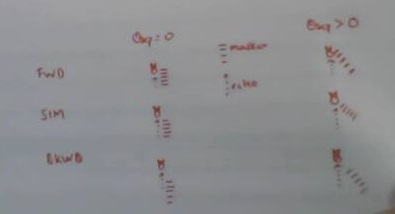
\includegraphics{img/masking_types.jpg} \#\#\# Though there are these 6
possible kinds of echo-masker configurations - we still have a set of
parameters undefined : \#\#\# 1) Relative intensities of echo and masker
\#\#\# 2) Time ranges over which forward/backward masking occur \#\#\#
3) \(\theta_{separation}\) at which spatial unmasking begins to occur

    \hypertarget{a-quick-literature-survey}{%
\section{A Quick Literature Survey :}\label{a-quick-literature-survey}}

\hypertarget{there-are-a-bunch-of-studies-which-have-either-actively-investigated-masking-or-where-masking-occurs-as-part-of-the-study-design.-i-looked-into-the-bat-psychoacoustics-literature-to-get-some-estimates-of-the-above-parameters-in-each-case-presented-here-as-a-table.}{%
\subsection{There are a bunch of studies which have either actively
investigated masking, or where masking occurs as part of the study
design. I looked into the bat psychoacoustics literature to get some
estimates of the above parameters in each case, presented here as a
table.}\label{there-are-a-bunch-of-studies-which-have-either-actively-investigated-masking-or-where-masking-occurs-as-part-of-the-study-design.-i-looked-into-the-bat-psychoacoustics-literature-to-get-some-estimates-of-the-above-parameters-in-each-case-presented-here-as-a-table.}}

\hypertarget{here-it-is-important-to-note-that-when-i-use-the-terms-forward-or-backward-masking-i-also-include-situations-where-there-is-echomasker-overlap.-for-eg.-when-a-masker-arrived-before-an-echo-and-then-overlaps-it-also---i-still-refer-to-this-as-forward-masking.-typically-one-would-refer-to-forwardbackward-masking-when-there-is-no-overlap-at-all.}{%
\subsection{Here it is important to note that when I use the terms
`forward' or `backward' masking I also include situations where there is
echo+masker overlap. For eg. when a masker arrived before an echo, and
then overlaps it also - I still refer to this as `forward' masking.
Typically, one would refer to forward/backward masking when there is no
overlap at
all.}\label{here-it-is-important-to-note-that-when-i-use-the-terms-forward-or-backward-masking-i-also-include-situations-where-there-is-echomasker-overlap.-for-eg.-when-a-masker-arrived-before-an-echo-and-then-overlaps-it-also---i-still-refer-to-this-as-forward-masking.-typically-one-would-refer-to-forwardbackward-masking-when-there-is-no-overlap-at-all.}}

    \begin{Verbatim}[commandchars=\\\{\}]
{\color{incolor}In [{\color{incolor}4}]:} \PY{n}{table\PYZus{}wrefs} \PY{o}{=} \PY{p}{[}\PY{p}{[} \PY{l+s+s1}{\PYZsq{}}\PY{l+s+s1}{1) \PYZdl{}}\PY{l+s+se}{\PYZbs{}\PYZbs{}}\PY{l+s+s1}{theta\PYZus{}\PYZob{}separation\PYZcb{} = 0 + Forward}\PY{l+s+s1}{\PYZbs{}}\PY{l+s+s1}{ masking\PYZdl{} : Miller 1991, Ruihong et al. 2003,}\PY{l+s+se}{\PYZbs{}}
        \PY{l+s+s1}{                chp 36 Siewert et al. Echolocation in Dolphins and Bats}\PY{l+s+s1}{\PYZsq{}}\PY{p}{,}
        \PY{l+s+s1}{\PYZsq{}}\PY{l+s+s1}{2) \PYZdl{}}\PY{l+s+se}{\PYZbs{}\PYZbs{}}\PY{l+s+s1}{theta\PYZus{}\PYZob{}separation\PYZcb{} \PYZgt{}0\PYZdl{} + \PYZdl{}Forward}\PY{l+s+s1}{\PYZbs{}}\PY{l+s+s1}{ masking\PYZdl{}: ????}\PY{l+s+s1}{\PYZsq{}}\PY{p}{]}\PY{p}{,}              
        \PY{p}{[} \PY{l+s+s1}{\PYZsq{}}\PY{l+s+s1}{3) \PYZdl{}}\PY{l+s+se}{\PYZbs{}\PYZbs{}}\PY{l+s+s1}{theta\PYZus{}\PYZob{}separation\PYZcb{} = 0\PYZdl{} + \PYZdl{}Simultaneous}\PY{l+s+s1}{\PYZbs{}}\PY{l+s+s1}{ masking\PYZdl{}:  Troest \PYZam{} Mohl 1986}\PY{l+s+s1}{\PYZsq{}}\PY{p}{,}
         \PY{l+s+s1}{\PYZsq{}}\PY{l+s+s1}{4) \PYZdl{}}\PY{l+s+se}{\PYZbs{}\PYZbs{}}\PY{l+s+s1}{theta\PYZus{}\PYZob{}separation\PYZcb{} \PYZgt{}0\PYZdl{} + \PYZdl{}Simultaneous}\PY{l+s+s1}{\PYZbs{}}\PY{l+s+s1}{ masking\PYZdl{}: Warnecke et al. 2014, \PYZdl{}}\PY{l+s+se}{\PYZbs{}\PYZbs{}}\PY{l+s+s1}{theta\PYZus{}\PYZob{}separation\PYZcb{}\PYZdl{} = \PYZdl{}90\PYZca{}\PYZob{}}\PY{l+s+s1}{\PYZbs{}}\PY{l+s+s1}{circ\PYZcb{}\PYZdl{}}\PY{l+s+s1}{\PYZsq{}}\PY{p}{]}\PY{p}{,}
        \PY{p}{[}\PY{l+s+s1}{\PYZsq{}}\PY{l+s+s1}{5) \PYZdl{}}\PY{l+s+se}{\PYZbs{}\PYZbs{}}\PY{l+s+s1}{theta\PYZus{}\PYZob{}separation\PYZcb{} = 0\PYZdl{} + \PYZdl{}Backward}\PY{l+s+s1}{\PYZbs{}}\PY{l+s+s1}{ masking\PYZdl{}: Suemer et al. 2009,Mohl and Surlykke 1989}\PY{l+s+s1}{\PYZsq{}}\PY{p}{,}
         \PY{l+s+s1}{\PYZsq{}}\PY{l+s+s1}{6) \PYZdl{}}\PY{l+s+se}{\PYZbs{}\PYZbs{}}\PY{l+s+s1}{theta\PYZus{}\PYZob{}separation\PYZcb{} \PYZgt{}0\PYZdl{} + \PYZdl{}Backward}\PY{l+s+s1}{\PYZbs{}}\PY{l+s+s1}{ masking\PYZdl{}: Suemer et al. 2009, \PYZdl{}}\PY{l+s+se}{\PYZbs{}\PYZbs{}}\PY{l+s+s1}{theta\PYZus{}\PYZob{}separation\PYZcb{}\PYZdl{}: \PYZdl{}0\PYZhy{} 23\PYZca{}\PYZob{}}\PY{l+s+s1}{\PYZbs{}}\PY{l+s+s1}{circ\PYZcb{}\PYZdl{}}\PY{l+s+s1}{\PYZsq{}}\PY{p}{]}\PY{p}{]}
        \PY{n}{display}\PY{p}{(}\PY{n}{HTML}\PY{p}{(}\PY{n}{tabulate}\PY{o}{.}\PY{n}{tabulate}\PY{p}{(}\PY{n}{table\PYZus{}wrefs}\PY{p}{,}\PY{n}{tablefmt}\PY{o}{=}\PY{l+s+s1}{\PYZsq{}}\PY{l+s+s1}{html}\PY{l+s+s1}{\PYZsq{}}\PY{p}{)}\PY{p}{)}\PY{p}{)}
\end{Verbatim}

    
    \begin{verbatim}
<IPython.core.display.HTML object>
    \end{verbatim}

    
    \hypertarget{following-this-broad-summary-of-the-studies-with-various-parameters-let-us-now-take-a-look-at-the-range-of-values-reported-in-the-studies}{%
\subsection{Following this broad summary of the studies with various
parameters, let us now take a look at the range of values reported in
the
studies:}\label{following-this-broad-summary-of-the-studies-with-various-parameters-let-us-now-take-a-look-at-the-range-of-values-reported-in-the-studies}}

\hypertarget{theta_separation0-forward-masking}{%
\subsection{\texorpdfstring{1)
\emph{\(\theta_{separation}=0 + Forward\ masking\) :
}}{1) \textbackslash{}theta\_\{separation\}=0 + Forward\textbackslash{} masking : }}\label{theta_separation0-forward-masking}}

\hypertarget{miller-1991-studied-how-ultrasonic-clicking-of-moths-may-affect-preyobject-ranging-in-echolocating-bats.-ultrasonic-clicks-were-played-back-when-triggered-by-the-bats-calls-and-were-timed-to-arrive-within-a-particular-time-delay-of-a-phantom-echo.-bats-were-trained-to-distinguish-between-two-echoes-a-near-and-far-phantom-echoes---and-had-to-indicate-the-echo-type-on-playback.-the-clicks-and-echoes-were-presented-from-the-same-speaker.}{%
\subsubsection{\texorpdfstring{\textgreater{}
\href{https://link.springer.com/article/10.1007/BF00215079}{\(Miller\ 1991\)}
: studied how ultrasonic clicking of moths may affect prey/object
ranging in echolocating bats. Ultrasonic clicks were played back when
triggered by the bat's calls and were timed to arrive within a
particular time delay of a phantom echo. Bats were trained to
distinguish between two echoes, a `near' and `far' phantom echoes - and
had to indicate the echo type on playback. The clicks and echoes were
presented from the same
speaker.}{\textgreater{} Miller\textbackslash{} 1991 : studied how ultrasonic clicking of moths may affect prey/object ranging in echolocating bats. Ultrasonic clicks were played back when triggered by the bat's calls and were timed to arrive within a particular time delay of a phantom echo. Bats were trained to distinguish between two echoes, a `near' and `far' phantom echoes - and had to indicate the echo type on playback. The clicks and echoes were presented from the same speaker.}}\label{miller-1991-studied-how-ultrasonic-clicking-of-moths-may-affect-preyobject-ranging-in-echolocating-bats.-ultrasonic-clicks-were-played-back-when-triggered-by-the-bats-calls-and-were-timed-to-arrive-within-a-particular-time-delay-of-a-phantom-echo.-bats-were-trained-to-distinguish-between-two-echoes-a-near-and-far-phantom-echoes---and-had-to-indicate-the-echo-type-on-playback.-the-clicks-and-echoes-were-presented-from-the-same-speaker.}}

\hypertarget{when-clicks-arrived-within-1.5-milliseconds-of-the-phantom-echo-the-bats-could-not-distinguish-between-the-far-and-the-near-echo-types-properly.-this-may-indicate-some-kind-of-masking-that-occured-at-these-echo-click-delays.}{%
\subsubsection{\texorpdfstring{When clicks arrived within 1.5
milliseconds of the phantom echo, the bats could not distinguish between
the `far' and the `near' echo types properly. This \emph{may} indicate
some kind of masking that occured at these echo-click
delays.}{When clicks arrived within 1.5 milliseconds of the phantom echo, the bats could not distinguish between the `far' and the `near' echo types properly. This may indicate some kind of masking that occured at these echo-click delays.}}\label{when-clicks-arrived-within-1.5-milliseconds-of-the-phantom-echo-the-bats-could-not-distinguish-between-the-far-and-the-near-echo-types-properly.-this-may-indicate-some-kind-of-masking-that-occured-at-these-echo-click-delays.}}

\hypertarget{caveats-to-consider-the-study-results-may-also-be-the-result-of-further-masking-from-the-clutter-echoes-as-in-some-experimental-treatments-there-was-temporal-overlap-of-the-phantom-echoes-and-clicks-with-the-echo-from-the-loudspeaker.}{%
\subsubsection{Caveats to consider: the study results may also be the
result of further masking from the clutter echoes as in some
experimental treatments there was temporal overlap of the phantom echoes
and clicks with the echo from the
loudspeaker.}\label{caveats-to-consider-the-study-results-may-also-be-the-result-of-further-masking-from-the-clutter-echoes-as-in-some-experimental-treatments-there-was-temporal-overlap-of-the-phantom-echoes-and-clicks-with-the-echo-from-the-loudspeaker.}}

\hypertarget{echo-level-68-db-pespl-re-20mupa}{%
\subsubsection{\texorpdfstring{Echo level : 68 dB peSPL re
20\(\mu\)Pa}{Echo level : 68 dB peSPL re 20\textbackslash{}muPa}}\label{echo-level-68-db-pespl-re-20mupa}}

\hypertarget{masker-click-level-64-db-pespl-calculated.}{%
\subsubsection{Masker (click) level: 64 dB peSPL
(calculated).}\label{masker-click-level-64-db-pespl-calculated.}}

\hypertarget{masking-time-range-1.5-milliseconds.}{%
\subsubsection{Masking time range : \textless{}=1.5
milliseconds.}\label{masking-time-range-1.5-milliseconds.}}

\hypertarget{delta-target-masker-db-spl-68---64-4-db}{%
\subsubsection{\texorpdfstring{\(\Delta\) target-masker dB SPL : 68 - 64
= 4
dB}{\textbackslash{}Delta target-masker dB SPL : 68 - 64 = 4 dB}}\label{delta-target-masker-db-spl-68---64-4-db}}

\hypertarget{study-species-eptesicus-fuscus}{%
\subsubsection{\texorpdfstring{Study species : \emph{Eptesicus
fuscus}}{Study species : Eptesicus fuscus}}\label{study-species-eptesicus-fuscus}}

\hypertarget{ruihong-et-al.-2003-studied-how-neurons-in-the-inferior-colliculus-ic-respond-to-the-presence-of-a-loud-sound-that-preced-the-target-sound.-this-is-somewhat-analogous-to-forward-masking-in-psychoacoustics.-the-masker-and-the-target-were-sinusoids-of-the-best-frequency-of-the-probed-neuron.-when-the-time-gap-between-the-masker-and-the-target-sound-increased-beyond-3-milliseconds-the-response-of-the-ic-neurons-increased.-when-the-masker-and-target-were-close-in-time-there-was-a-suppression-in-neuronal-activity-seen.-the-masker-was-presented-at-1020-30-db-above-the-minimum-threshold-and-the-time-gaps-between-the-masker-and-target-were-also-varied-between-1369-and-12-milliseconds.}{%
\subsubsection{\texorpdfstring{\textgreater{}
\href{https://link.springer.com/article/10.1360/02wc0570}{\(Ruihong\ et\ al.\ 2003\)}
: studied how neurons in the Inferior Colliculus (IC) respond to the
presence of a loud sound that preced the target sound. This is somewhat
analogous to forward masking in psychoacoustics. The masker and the
target were sinusoids of the best frequency of the probed neuron. When
the time gap between the `masker' and the `target' sound increased
beyond 3 milliseconds, the response of the IC neurons increased. When
the masker and target were close in time, there was a `suppression' in
neuronal activity seen. The masker was presented at 10,20 \& 30 dB above
the minimum threshold, and the time gaps between the masker and target
were also varied between 1,3,6,9 and 12
milliseconds.}{\textgreater{} Ruihong\textbackslash{} et\textbackslash{} al.\textbackslash{} 2003 : studied how neurons in the Inferior Colliculus (IC) respond to the presence of a loud sound that preced the target sound. This is somewhat analogous to forward masking in psychoacoustics. The masker and the target were sinusoids of the best frequency of the probed neuron. When the time gap between the `masker' and the `target' sound increased beyond 3 milliseconds, the response of the IC neurons increased. When the masker and target were close in time, there was a `suppression' in neuronal activity seen. The masker was presented at 10,20 \& 30 dB above the minimum threshold, and the time gaps between the masker and target were also varied between 1,3,6,9 and 12 milliseconds.}}\label{ruihong-et-al.-2003-studied-how-neurons-in-the-inferior-colliculus-ic-respond-to-the-presence-of-a-loud-sound-that-preced-the-target-sound.-this-is-somewhat-analogous-to-forward-masking-in-psychoacoustics.-the-masker-and-the-target-were-sinusoids-of-the-best-frequency-of-the-probed-neuron.-when-the-time-gap-between-the-masker-and-the-target-sound-increased-beyond-3-milliseconds-the-response-of-the-ic-neurons-increased.-when-the-masker-and-target-were-close-in-time-there-was-a-suppression-in-neuronal-activity-seen.-the-masker-was-presented-at-1020-30-db-above-the-minimum-threshold-and-the-time-gaps-between-the-masker-and-target-were-also-varied-between-1369-and-12-milliseconds.}}

\hypertarget{caveats-to-consider-this-study-was-done-on-anesthetised-bats-and-playbacks-were-done-monaurally.-it-may-also-be-difficult-to-interpret-the-ic-neuron-response-in-terms-of-what-the-bat-may-actually-experience-perceptually-the-target-sound-was-also-a-single-frequency-tone-rather-than-a-echolocation-like-call.}{%
\subsubsection{Caveats to consider: This study was done on anesthetised
bats, and playbacks were done monaurally. It may also be difficult to
interpret the IC neuron response in terms of what the bat may actually
experience perceptually? The `target' sound was also a single frequency
tone, rather than a echolocation-like
call.}\label{caveats-to-consider-this-study-was-done-on-anesthetised-bats-and-playbacks-were-done-monaurally.-it-may-also-be-difficult-to-interpret-the-ic-neuron-response-in-terms-of-what-the-bat-may-actually-experience-perceptually-the-target-sound-was-also-a-single-frequency-tone-rather-than-a-echolocation-like-call.}}

\hypertarget{target-sound-level-varying---depends-on-the-neuronal-unit-being-measured}{%
\subsubsection{Target sound level: varying - depends on the neuronal
unit being
measured}\label{target-sound-level-varying---depends-on-the-neuronal-unit-being-measured}}

\hypertarget{masker-level-1020-30-db-above-the-minimum-threshold-level}{%
\subsubsection{Masker level: 10,20 \& 30 dB above the minimum threshold
level}\label{masker-level-1020-30-db-above-the-minimum-threshold-level}}

\hypertarget{masking-time-range-3-milliseconds.}{%
\subsubsection{Masking time range : \textless{}=3
milliseconds.}\label{masking-time-range-3-milliseconds.}}

\hypertarget{study-species-eptesicus-fuscus-1}{%
\subsubsection{\texorpdfstring{Study species: \emph{Eptesicus
fuscus}}{Study species: Eptesicus fuscus}}\label{study-species-eptesicus-fuscus-1}}

\hypertarget{delta-target-masker-db-spl--10--20--30-db-depending-on-the-playback-level}{%
\subsubsection{\texorpdfstring{\(\Delta\) target-masker dB SPL : -10,
-20, -30 dB, depending on the playback
level}{\textbackslash{}Delta target-masker dB SPL : -10, -20, -30 dB, depending on the playback level}}\label{delta-target-masker-db-spl--10--20--30-db-depending-on-the-playback-level}}

\hypertarget{siewert-et-al.-2004-chapter-36-bats-were-trained-to-fly-towards-a-speaker-playing-back-a-test-signal.-the-test-signal-was-a-megaderma-lyra-multiharmonic-approach-call.-the-test-signal-was-played-back-in-the-presence-of-broadband-noise-with-decreasing-power-from-10-100-khz.-in-experiment-2-the-delay-between-the-end-of-the-broadband-noise-and-start-of-the-test-signal-was-varied-between-24-to--6-ms.-the-noise-pulse-was-40-milliseconds-long.-the-same-hearing-thresholds-as-reached-under-no-noise-conditions-was-reached-at-30-40-ms.-in-our-experiment-the-detection-thresholds-increased-by-about-6-db-per-delay-half-reduction.}{%
\subsubsection{\texorpdfstring{\textgreater{}
\href{http://press.uchicago.edu/ucp/books/book/chicago/E/bo3612864.html}{\(Siewert\ et\ al.\ 2004\, (chapter\ 36)\)}:
Bats were trained to fly towards a speaker playing back a test signal.
The test signal was a \emph{Megaderma lyra} multiharmonic approach call.
The test signal was played back in the presence of broadband noise with
decreasing power from 10-100 KHz. In Experiment 2, the delay between the
end of the broadband noise and start of the test signal was varied
between 24 to -6 ms. The noise pulse was 40 milliseconds long. The same
hearing thresholds as reached under no noise conditions was reached at
30-40 ms. \emph{`In our experiment, the detection thresholds increased
by about 6 dB per delay half
reduction'.}}{\textgreater{} Siewert\textbackslash{} et\textbackslash{} al.\textbackslash{} 2004\textbackslash{}, (chapter\textbackslash{} 36): Bats were trained to fly towards a speaker playing back a test signal. The test signal was a Megaderma lyra multiharmonic approach call. The test signal was played back in the presence of broadband noise with decreasing power from 10-100 KHz. In Experiment 2, the delay between the end of the broadband noise and start of the test signal was varied between 24 to -6 ms. The noise pulse was 40 milliseconds long. The same hearing thresholds as reached under no noise conditions was reached at 30-40 ms. `In our experiment, the detection thresholds increased by about 6 dB per delay half reduction'.}}\label{siewert-et-al.-2004-chapter-36-bats-were-trained-to-fly-towards-a-speaker-playing-back-a-test-signal.-the-test-signal-was-a-megaderma-lyra-multiharmonic-approach-call.-the-test-signal-was-played-back-in-the-presence-of-broadband-noise-with-decreasing-power-from-10-100-khz.-in-experiment-2-the-delay-between-the-end-of-the-broadband-noise-and-start-of-the-test-signal-was-varied-between-24-to--6-ms.-the-noise-pulse-was-40-milliseconds-long.-the-same-hearing-thresholds-as-reached-under-no-noise-conditions-was-reached-at-30-40-ms.-in-our-experiment-the-detection-thresholds-increased-by-about-6-db-per-delay-half-reduction.}}

\hypertarget{target-sound-level-graphical-estimates-with-db-rounded-off-to-closest-integer-value}{%
\subsubsection{Target sound level: (graphical estimates, with dB rounded
off to closest integer
value)}\label{target-sound-level-graphical-estimates-with-db-rounded-off-to-closest-integer-value}}

\begin{longtable}[]{@{}ll@{}}
\toprule
Masker-echo delay (milliseconds) & Echo level (dB SPL)\tabularnewline
\midrule
\endhead
3 & 28\tabularnewline
6 & 22\tabularnewline
12 & 16\tabularnewline
24 & 11\tabularnewline
\bottomrule
\end{longtable}

\hypertarget{masker-sound-level-45-db-spl}{%
\subsubsection{Masker sound level: 45 dB
SPL}\label{masker-sound-level-45-db-spl}}

\hypertarget{masking-time-range-tested-for-upto-24-ms}{%
\subsubsection{Masking time range: tested for upto 24
ms}\label{masking-time-range-tested-for-upto-24-ms}}

\hypertarget{delta-target-masker-db-spl}{%
\subsubsection{\texorpdfstring{\(\Delta\) target-masker dB
SPL:}{\textbackslash{}Delta target-masker dB SPL:}}\label{delta-target-masker-db-spl}}

\begin{longtable}[]{@{}ll@{}}
\toprule
Masker-echo delay (milliseconds) & \(\Delta\) dB SPL echo to noise
(dB)\tabularnewline
\midrule
\endhead
3 & -17\tabularnewline
6 & -23\tabularnewline
12 & -29\tabularnewline
24 & -34\tabularnewline
\bottomrule
\end{longtable}

\hypertarget{study-species-megaderma-lyra}{%
\subsubsection{\texorpdfstring{Study species: \emph{Megaderma
lyra}}{Study species: Megaderma lyra}}\label{study-species-megaderma-lyra}}

\hypertarget{caveats-to-consider}{%
\subsubsection{Caveats to consider: ?}\label{caveats-to-consider}}

    

    \hypertarget{theta_separation0-forward-masking}{%
\subsection{\texorpdfstring{2)
\emph{\(\theta_{separation}>0 + Forward\ masking\) :
}}{2) \textbackslash{}theta\_\{separation\}\textgreater{}0 + Forward\textbackslash{} masking : }}\label{theta_separation0-forward-masking}}

\hypertarget{as-of-now-have-not-been-able-to-find-relevant-papers}{%
\subsection{\texorpdfstring{\emph{As of now, have not been able to find
relevant
papers}}{As of now, have not been able to find relevant papers}}\label{as-of-now-have-not-been-able-to-find-relevant-papers}}

    \hypertarget{theta_separation-0-simultaneous-masking}{%
\subsection{\texorpdfstring{3) \emph{\(\theta_{separation} = 0\) +
\(Simultaneous\ masking\)}}{3) \textbackslash{}theta\_\{separation\} = 0 + Simultaneous\textbackslash{} masking}}\label{theta_separation-0-simultaneous-masking}}

\hypertarget{troest-and-mohl-1986-bats-were-trained-to-tell-if-there-was-a-phantom-echo-present-or-not-by-moving-to-one-side-of-a-two-choice-setup.-noise-and-phantom-echoes-were-played-from-a-single-speaker.-the-noise-was-a-broadband-white-noise-with-power-spectral-density-of--113-db-re-1-fracpasqrthz-and-the-phantom-echo-was-a-replicate-of-the-bat-call.}{%
\subsubsection{\texorpdfstring{\textgreater{}\href{https://link.springer.com/article/10.1007\%2FBF00604175?LI=true}{\(Troest\ and\ Mohl\ 1986\)}:
Bats were trained to tell if there was a phantom echo present or not by
moving to one side of a two choice setup. Noise and phantom echoes were
played from a single speaker. The noise was a broadband white noise with
power spectral density of \(-113\ dB\ re\ 1\ \frac{Pa}{\sqrt{Hz}}\), and
the phantom echo was a replicate of the bat
call.}{\textgreater{}Troest\textbackslash{} and\textbackslash{} Mohl\textbackslash{} 1986: Bats were trained to tell if there was a phantom echo present or not by moving to one side of a two choice setup. Noise and phantom echoes were played from a single speaker. The noise was a broadband white noise with power spectral density of -113\textbackslash{} dB\textbackslash{} re\textbackslash{} 1\textbackslash{} \textbackslash{}frac\{Pa\}\{\textbackslash{}sqrt\{Hz\}\}, and the phantom echo was a replicate of the bat call.}}\label{troest-and-mohl-1986-bats-were-trained-to-tell-if-there-was-a-phantom-echo-present-or-not-by-moving-to-one-side-of-a-two-choice-setup.-noise-and-phantom-echoes-were-played-from-a-single-speaker.-the-noise-was-a-broadband-white-noise-with-power-spectral-density-of--113-db-re-1-fracpasqrthz-and-the-phantom-echo-was-a-replicate-of-the-bat-call.}}

\hypertarget{target-phantom-echo-level-without-noise-40-48-db-pespl-re-20mupa-with-noise-47-58-db-pespl-delta-increase-of-7-10-db-pespl-in-the-presence-of-noise.}{%
\subsubsection{\texorpdfstring{Target phantom echo level: without noise:
40-48 dB peSPL re 20\(\mu\)Pa , \emph{with noise} : 47-58 dB peSPL,
\(\Delta\) increase of 7-10 dB peSPL in the presence of
noise.}{Target phantom echo level: without noise: 40-48 dB peSPL re 20\textbackslash{}muPa , with noise : 47-58 dB peSPL, \textbackslash{}Delta increase of 7-10 dB peSPL in the presence of noise.}}\label{target-phantom-echo-level-without-noise-40-48-db-pespl-re-20mupa-with-noise-47-58-db-pespl-delta-increase-of-7-10-db-pespl-in-the-presence-of-noise.}}

\hypertarget{masker-sound-level-55-db-pe-spl-calculated}{%
\subsubsection{Masker sound level: 55 dB pe SPL
(calculated)}\label{masker-sound-level-55-db-pe-spl-calculated}}

\hypertarget{masking-time-range-not-valid-simultaneous-masking}{%
\subsubsection{Masking time range: NOT VALID, simultaneous
masking}\label{masking-time-range-not-valid-simultaneous-masking}}

\hypertarget{study-species-eptesicus-serotinus}{%
\subsubsection{\texorpdfstring{Study species: \emph{Eptesicus
serotinus}}{Study species: Eptesicus serotinus}}\label{study-species-eptesicus-serotinus}}

\hypertarget{caveats-to-consider}{%
\subsubsection{Caveats to consider: ?}\label{caveats-to-consider}}

\hypertarget{delta-target-masker-db-spl-47-58---55--8-to-3-db}{%
\subsubsection{\texorpdfstring{\(\Delta\) target-masker dB SPL : 47-58 -
55 = -8 to +3
dB}{\textbackslash{}Delta target-masker dB SPL : 47-58 - 55 = -8 to +3 dB}}\label{delta-target-masker-db-spl-47-58---55--8-to-3-db}}

\hypertarget{mohl-and-surlykke-1989-bats-were-trained-to-tell-if-there-was-a-phantom-echo-present-or-not-in-the-presence-of-a-noise-signal-that-varied-in-delay.-simultaneous-to-backward-masking-situations-were-investigated.}{%
\subsubsection{\texorpdfstring{\textgreater{}\href{https://link.springer.com/article/10.1007\%2FBF00613805?LI=true}{\(Mohl\ and\ Surlykke\ 1989\)}:
Bats were trained to tell if there was a phantom echo present or not in
the presence of a noise signal that varied in delay. Simultaneous to
backward masking situations were
investigated.}{\textgreater{}Mohl\textbackslash{} and\textbackslash{} Surlykke\textbackslash{} 1989: Bats were trained to tell if there was a phantom echo present or not in the presence of a noise signal that varied in delay. Simultaneous to backward masking situations were investigated.}}\label{mohl-and-surlykke-1989-bats-were-trained-to-tell-if-there-was-a-phantom-echo-present-or-not-in-the-presence-of-a-noise-signal-that-varied-in-delay.-simultaneous-to-backward-masking-situations-were-investigated.}}

\hypertarget{for-simultaneous-masking-experiments-the-noise-was-broadband-with--5-db-fracsplsqrthz-with-durations-of-2-37.5-milliseconds.}{%
\subsubsection{\texorpdfstring{For simultaneous masking experiments the
noise was broadband with \(-5\ dB\ \frac{SPL}{\sqrt(Hz)}\) with
durations of 2-37.5
milliseconds.}{For simultaneous masking experiments the noise was broadband with -5\textbackslash{} dB\textbackslash{} \textbackslash{}frac\{SPL\}\{\textbackslash{}sqrt(Hz)\} with durations of 2-37.5 milliseconds.}}\label{for-simultaneous-masking-experiments-the-noise-was-broadband-with--5-db-fracsplsqrthz-with-durations-of-2-37.5-milliseconds.}}

\hypertarget{simulatenous-masking-was-also-tested-at-the-the-zero-delay-of-the-backward-masking-experiments-a-broadband-noise-with-16-db-fracsplsqrthz-power-spectral-density-was-used-of-5-milliseconds.}{%
\subsubsection{\texorpdfstring{Simulatenous masking was also tested at
the the zero delay of the backward masking experiments, a broadband
noise with \(16\ dB\ \frac{SPL}{\sqrt(Hz)}\) power spectral density was
used of 5
milliseconds.}{Simulatenous masking was also tested at the the zero delay of the backward masking experiments, a broadband noise with 16\textbackslash{} dB\textbackslash{} \textbackslash{}frac\{SPL\}\{\textbackslash{}sqrt(Hz)\} power spectral density was used of 5 milliseconds.}}\label{simulatenous-masking-was-also-tested-at-the-the-zero-delay-of-the-backward-masking-experiments-a-broadband-noise-with-16-db-fracsplsqrthz-power-spectral-density-was-used-of-5-milliseconds.}}

\hypertarget{simultaneous-masking-experiment-results}{%
\subsubsection{\texorpdfstring{\emph{simultaneous masking experiment
results:}}{simultaneous masking experiment results:}}\label{simultaneous-masking-experiment-results}}

\hypertarget{target-phantom-echo-level-without-noise37-38-db-spl-re-20mupa-with-noise-adding-15-db-52-53-db-pespl-delta-increase-of-15-db-in-the-presence-of-noise.}{%
\subsubsection{\texorpdfstring{Target phantom echo level: without
noise:37-38 dB SPL re 20\(\mu\)Pa , \emph{with noise} : (adding 15 dB)
52-53 dB peSPL, \(\Delta\) increase of 15 dB in the presence of
noise.}{Target phantom echo level: without noise:37-38 dB SPL re 20\textbackslash{}muPa , with noise : (adding 15 dB) 52-53 dB peSPL, \textbackslash{}Delta increase of 15 dB in the presence of noise.}}\label{target-phantom-echo-level-without-noise37-38-db-spl-re-20mupa-with-noise-adding-15-db-52-53-db-pespl-delta-increase-of-15-db-in-the-presence-of-noise.}}

\hypertarget{masker-sound-level-to-be-calculated}{%
\subsubsection{\texorpdfstring{Masker sound level: \emph{to be
calculated}}{Masker sound level: to be calculated}}\label{masker-sound-level-to-be-calculated}}

\hypertarget{zero-delay-of-backward-masking-experiment-results}{%
\subsubsection{\texorpdfstring{\emph{zero delay of backward masking
experiment
results:}}{zero delay of backward masking experiment results:}}\label{zero-delay-of-backward-masking-experiment-results}}

\hypertarget{target-phantom-echo-level-without-noise37-38-db-spl-re-20mupa-with-noise-adding-35-db-72-73-db-pespl-delta-increase-of-35-db-in-the-presence-of-noise-graphical-estimate.}{%
\subsubsection{\texorpdfstring{Target phantom echo level: without
noise:37-38 dB SPL re 20\(\mu\)Pa , \emph{with noise} : (adding
\textasciitilde{}35 dB) 72-73 dB peSPL, \(\Delta\) increase of 35 dB in
the presence of noise (graphical
estimate).}{Target phantom echo level: without noise:37-38 dB SPL re 20\textbackslash{}muPa , with noise : (adding \textasciitilde{}35 dB) 72-73 dB peSPL, \textbackslash{}Delta increase of 35 dB in the presence of noise (graphical estimate).}}\label{target-phantom-echo-level-without-noise37-38-db-spl-re-20mupa-with-noise-adding-35-db-72-73-db-pespl-delta-increase-of-35-db-in-the-presence-of-noise-graphical-estimate.}}

\hypertarget{masker-sound-level-to-be-calculated-1}{%
\subsubsection{\texorpdfstring{Masker sound level: \emph{to be
calculated}}{Masker sound level: to be calculated}}\label{masker-sound-level-to-be-calculated-1}}

\hypertarget{masking-time-range-not-valid-simultaneous-masking-1}{%
\subsubsection{Masking time range: NOT VALID, simultaneous
masking}\label{masking-time-range-not-valid-simultaneous-masking-1}}

\hypertarget{study-species-eptesicus-serotinus-1}{%
\subsubsection{\texorpdfstring{Study species: \emph{Eptesicus
serotinus}}{Study species: Eptesicus serotinus}}\label{study-species-eptesicus-serotinus-1}}

\hypertarget{caveats-to-consider-1}{%
\subsubsection{Caveats to consider: ?}\label{caveats-to-consider-1}}

\hypertarget{siewert-et-al.-2004-chapter-36-see-1-for-experiment-description.-there-was-a-complete-overlap-of-test-signal-and-noise-at-the--6-millisconds-delay-between-noise-and-test-signal-the-experiment-looked-at-simultaneous-masking.}{%
\subsubsection{\texorpdfstring{\textgreater{}
\href{http://press.uchicago.edu/ucp/books/book/chicago/E/bo3612864.html}{\(Siewert\ et\ al.\ 2004\, (chapter\ 36)\)}:
See 1) for experiment description. There was a complete overlap of test
signal and noise at the -6 millisconds delay between noise and test
signal, the experiment looked at simultaneous
masking.}{\textgreater{} Siewert\textbackslash{} et\textbackslash{} al.\textbackslash{} 2004\textbackslash{}, (chapter\textbackslash{} 36): See 1) for experiment description. There was a complete overlap of test signal and noise at the -6 millisconds delay between noise and test signal, the experiment looked at simultaneous masking.}}\label{siewert-et-al.-2004-chapter-36-see-1-for-experiment-description.-there-was-a-complete-overlap-of-test-signal-and-noise-at-the--6-millisconds-delay-between-noise-and-test-signal-the-experiment-looked-at-simultaneous-masking.}}

\hypertarget{milliseconds-delay-of-forward-masking-experiment-results}{%
\subsubsection{\texorpdfstring{\emph{-6 milliseconds delay of forward
masking experiment
results:}}{-6 milliseconds delay of forward masking experiment results:}}\label{milliseconds-delay-of-forward-masking-experiment-results}}

\hypertarget{target-phantom-echo-level-without-noise-for-2ms-test-signal-6.7-db-spl-re-20mupa-with-noise-36-db-splgraphical-estimate}{%
\subsubsection{\texorpdfstring{Target phantom echo level: without noise
(for 2ms test signal) : 6.7 dB SPL re 20\(\mu\)Pa , \emph{with noise}
:36 dB SPL(graphical
estimate),}{Target phantom echo level: without noise (for 2ms test signal) : 6.7 dB SPL re 20\textbackslash{}muPa , with noise :36 dB SPL(graphical estimate),}}\label{target-phantom-echo-level-without-noise-for-2ms-test-signal-6.7-db-spl-re-20mupa-with-noise-36-db-splgraphical-estimate}}

\hypertarget{delta-increase-of-29.3-db-in-the-presence-of-noise-.}{%
\subsubsection{\texorpdfstring{\(\Delta\) increase of 29.3 dB in the
presence of noise
.}{\textbackslash{}Delta increase of 29.3 dB in the presence of noise .}}\label{delta-increase-of-29.3-db-in-the-presence-of-noise-.}}

\hypertarget{masker-sound-level-45-db-spl}{%
\subsubsection{Masker sound level: 45 dB
SPL}\label{masker-sound-level-45-db-spl}}

\hypertarget{delta-target-masker-db-spl-36---45--9-db}{%
\subsubsection{\texorpdfstring{\(\Delta\) target-masker dB SPL : 36 - 45
= -9
dB}{\textbackslash{}Delta target-masker dB SPL : 36 - 45 = -9 dB}}\label{delta-target-masker-db-spl-36---45--9-db}}

    \hypertarget{theta_separation-0-simultaneous-masking}{%
\subsection{\texorpdfstring{4) \emph{\(\theta_{separation} >0\) +
\(Simultaneous\ masking\)}}{4) \textbackslash{}theta\_\{separation\} \textgreater{}0 + Simultaneous\textbackslash{} masking}}\label{theta_separation-0-simultaneous-masking}}

\hypertarget{warnecke-et-al.-2014-bats-were-trained-to-detect-a-target-echo-sound-played-from-either-a-left-or-right-speaker-set-at-a-fixed-angle-at-0-azimuth.-two-speakers-at-90-degrees-elevation-were-used-to-play-back-clutter-echoes-that-would-simultaneously-mask-the-target-echo.-all-combination-of-paired-clutter-echo-speaker-playbacks-were-carried-out-and-no-effect-was-seen-in-any-of-the-treatments.}{%
\subsubsection{\texorpdfstring{\textgreater{}\href{http://asa.scitation.org/doi/abs/10.1121/1.4869483}{\(Warnecke\ et\ al.\ 2014\)}:
Bats were trained to detect a target echo sound played from either a
left or right speaker set at a fixed angle at 0 azimuth. Two speakers at
90 degrees elevation were used to play back clutter echoes that would
simultaneously mask the target echo. All combination of paired
clutter-echo speaker playbacks were carried out, and no effect was seen
in any of the
treatments.}{\textgreater{}Warnecke\textbackslash{} et\textbackslash{} al.\textbackslash{} 2014: Bats were trained to detect a target echo sound played from either a left or right speaker set at a fixed angle at 0 azimuth. Two speakers at 90 degrees elevation were used to play back clutter echoes that would simultaneously mask the target echo. All combination of paired clutter-echo speaker playbacks were carried out, and no effect was seen in any of the treatments.}}\label{warnecke-et-al.-2014-bats-were-trained-to-detect-a-target-echo-sound-played-from-either-a-left-or-right-speaker-set-at-a-fixed-angle-at-0-azimuth.-two-speakers-at-90-degrees-elevation-were-used-to-play-back-clutter-echoes-that-would-simultaneously-mask-the-target-echo.-all-combination-of-paired-clutter-echo-speaker-playbacks-were-carried-out-and-no-effect-was-seen-in-any-of-the-treatments.}}

\hypertarget{target-phantom-echo-level-db-pespl-re-20mupa}{%
\subsubsection{\texorpdfstring{Target phantom echo level: ???? dB peSPL
re
20\(\mu\)Pa}{Target phantom echo level: ???? dB peSPL re 20\textbackslash{}muPa}}\label{target-phantom-echo-level-db-pespl-re-20mupa}}

\hypertarget{masker-level}{%
\subsubsection{Masker level: ??}\label{masker-level}}

\hypertarget{masking-time-range-not-valid-simultaneous-masking}{%
\subsubsection{Masking time range: NOT VALID, simultaneous
masking}\label{masking-time-range-not-valid-simultaneous-masking}}

\hypertarget{theta_separation-90circ-vertical-separation}{%
\subsubsection{\texorpdfstring{\(\theta_{separation}: >=90^{\circ}\)
vertical
separation}{\textbackslash{}theta\_\{separation\}: \textgreater{}=90\^{}\{\textbackslash{}circ\} vertical separation}}\label{theta_separation-90circ-vertical-separation}}

\hypertarget{study-species-eptesicus-fuscus}{%
\subsubsection{\texorpdfstring{Study species: \emph{Eptesicus
fuscus}}{Study species: Eptesicus fuscus}}\label{study-species-eptesicus-fuscus}}

    \hypertarget{theta_separation-0-backward-masking}{%
\subsection{\texorpdfstring{5) \(\theta_{separation} = 0\) +
\(Backward\ masking\)}{5) \textbackslash{}theta\_\{separation\} = 0 + Backward\textbackslash{} masking}}\label{theta_separation-0-backward-masking}}

\hypertarget{mohl-and-surlykke-1989-for-experiment-description-see-above-in-3.-in-backward-masking-experiments-the-noise-was-broadband-noise-with-power-spectral-density-of-16-db-fracsplsqrthz-of-5-millisecond-duration.-when-the-noise-followed-the-phantom-echo-beyond-2-milliseconds-the-bats-showed-similar-hearing-thresholds-as-the-reference-silence.}{%
\subsubsection{\texorpdfstring{\textgreater{}\href{https://link.springer.com/article/10.1007\%2FBF00613805?LI=true}{\(Mohl\ and\ Surlykke\ 1989\)}:
For experiment description see above in 3). In backward masking
experiments, the noise was broadband noise with power spectral density
of \(16\ dB\ \frac{SPL}{\sqrt(Hz)}\) of 5 millisecond duration. When the
noise followed the phantom echo beyond 2 milliseconds the bats showed
similar hearing thresholds as the reference
silence.}{\textgreater{}Mohl\textbackslash{} and\textbackslash{} Surlykke\textbackslash{} 1989: For experiment description see above in 3). In backward masking experiments, the noise was broadband noise with power spectral density of 16\textbackslash{} dB\textbackslash{} \textbackslash{}frac\{SPL\}\{\textbackslash{}sqrt(Hz)\} of 5 millisecond duration. When the noise followed the phantom echo beyond 2 milliseconds the bats showed similar hearing thresholds as the reference silence.}}\label{mohl-and-surlykke-1989-for-experiment-description-see-above-in-3.-in-backward-masking-experiments-the-noise-was-broadband-noise-with-power-spectral-density-of-16-db-fracsplsqrthz-of-5-millisecond-duration.-when-the-noise-followed-the-phantom-echo-beyond-2-milliseconds-the-bats-showed-similar-hearing-thresholds-as-the-reference-silence.}}

\hypertarget{target-phantom-echo-level-db-pespl-re-20mupa}{%
\subsubsection{\texorpdfstring{Target phantom echo level: ???? dB peSPL
re
20\(\mu\)Pa}{Target phantom echo level: ???? dB peSPL re 20\textbackslash{}muPa}}\label{target-phantom-echo-level-db-pespl-re-20mupa}}

\hypertarget{masker-sound-level-to-be-calculated}{%
\subsubsection{\texorpdfstring{Masker sound level: \emph{to be
calculated}}{Masker sound level: to be calculated}}\label{masker-sound-level-to-be-calculated}}

\hypertarget{masking-time-range-2-milliseconds}{%
\subsubsection{Masking time range: \textless{} 2
milliseconds}\label{masking-time-range-2-milliseconds}}

\hypertarget{study-species-eptesicus-fuscus}{%
\subsubsection{\texorpdfstring{Study species: \emph{Eptesicus
fuscus}}{Study species: Eptesicus fuscus}}\label{study-species-eptesicus-fuscus}}

\hypertarget{suxfcmeretal.2009-bats-were-trained-to-identify-if-a-target-echo-reflected-by-a-thin-wire-was-present-in-the-presence-of-a-masking-echo-big-flat-plate-which-arrived-soon-after-the-target-echo.-the-intensity-of-the-target-echo-was-varied-by-changing-the-diameter-of-the-wire-and-the-delay-of-the-masker-echo-was-varied-by-changing-its-distance-behind-the-target-wire.-all-thresholds-reported-here-are-for-the-75-correct-criterion.}{%
\subsubsection{\texorpdfstring{\textgreater{}\href{https://link.springer.com/article/10.1007/s00359-009-0424-9}{\$
Sümer~et~al.~2009\$}: Bats were trained to identify if a target echo
(reflected by a thin wire) was present in the presence of a masking echo
( big flat plate) which arrived soon after the target echo. The
intensity of the target echo was varied by changing the diameter of the
wire and the delay of the masker echo was varied by changing its
distance behind the target wire. All thresholds reported here are for
the 75\% correct
criterion.}{\textgreater{}\$ Sümer~et~al.~2009\$: Bats were trained to identify if a target echo (reflected by a thin wire) was present in the presence of a masking echo ( big flat plate) which arrived soon after the target echo. The intensity of the target echo was varied by changing the diameter of the wire and the delay of the masker echo was varied by changing its distance behind the target wire. All thresholds reported here are for the 75\% correct criterion.}}\label{suxfcmeretal.2009-bats-were-trained-to-identify-if-a-target-echo-reflected-by-a-thin-wire-was-present-in-the-presence-of-a-masking-echo-big-flat-plate-which-arrived-soon-after-the-target-echo.-the-intensity-of-the-target-echo-was-varied-by-changing-the-diameter-of-the-wire-and-the-delay-of-the-masker-echo-was-varied-by-changing-its-distance-behind-the-target-wire.-all-thresholds-reported-here-are-for-the-75-correct-criterion.}}

\hypertarget{caveats-to-consider-the-target-strength-measurements-reported-were-estimated-with-a-downward-sweep-playback.-most-speaker-constructions-have-a-limited-directionality-and-this-means-a-bat-may-perceive-much-higher-echo-levels-as-they-can-ensonify-greater-volumes-than-speakers-even-at-high-frequencies.}{%
\subsubsection{Caveats to consider: the target strength measurements
reported were estimated with a downward sweep playback. Most speaker
constructions have a limited directionality, and this means a bat may
perceive much higher echo levels as they can ensonify greater volumes
than speakers even at high
frequencies.}\label{caveats-to-consider-the-target-strength-measurements-reported-were-estimated-with-a-downward-sweep-playback.-most-speaker-constructions-have-a-limited-directionality-and-this-means-a-bat-may-perceive-much-higher-echo-levels-as-they-can-ensonify-greater-volumes-than-speakers-even-at-high-frequencies.}}

\hypertarget{target-echo-level-calculated-1.2mm-wire-had-target-strength-of--36.8-at-1m-distance.}{%
\subsubsection{Target echo level: (calculated) 1.2mm wire had target
strength of -36.8 at 1m
distance.}\label{target-echo-level-calculated-1.2mm-wire-had-target-strength-of--36.8-at-1m-distance.}}

\hypertarget{for-source-levels-of-97.9-105.2-db-pespl-10cm-this-is-77.9-85.2-db-pespl-1m-and-the-echo-levels-are-then}{%
\paragraph{For source levels of 97.9-105.2 dB peSPL (10cm), this is
77.9-85.2 dB peSPL (1m) , and the echo levels are
then:}\label{for-source-levels-of-97.9-105.2-db-pespl-10cm-this-is-77.9-85.2-db-pespl-1m-and-the-echo-levels-are-then}}

\hypertarget{db-pespl}{%
\subsubsection{41.1-68.4 dB peSPL}\label{db-pespl}}

\hypertarget{masker-sound-level}{%
\subsubsection{Masker sound level:}\label{masker-sound-level}}

\hypertarget{calculated-target-echo-level-22.3-db-which-is-then-in-the-range-of}{%
\paragraph{(calculated) target echo level + 22.3 dB, which is then in
the range
of}\label{calculated-target-echo-level-22.3-db-which-is-then-in-the-range-of}}

\hypertarget{db-pespl-1}{%
\subsubsection{63.4-90.7 dB peSPL}\label{db-pespl-1}}

\hypertarget{masking-time-range-0.65-milliseconds}{%
\subsubsection{Masking time range: \textless{} 0.65
milliseconds}\label{masking-time-range-0.65-milliseconds}}

\hypertarget{study-species-eptesicus-fuscus-1}{%
\subsubsection{\texorpdfstring{Study species: \emph{Eptesicus
fuscus}}{Study species: Eptesicus fuscus}}\label{study-species-eptesicus-fuscus-1}}

\hypertarget{delta-target-masker-db-spl--22.3-db}{%
\subsubsection{\texorpdfstring{\(\Delta\) target-masker dB SPL : -22.3
dB}{\textbackslash{}Delta target-masker dB SPL : -22.3 dB}}\label{delta-target-masker-db-spl--22.3-db}}

    \hypertarget{theta_separation-0-backward-masking}{%
\subsection{\texorpdfstring{6) \(\theta_{separation} >0\) + Backward
masking}{6) \textbackslash{}theta\_\{separation\} \textgreater{}0 + Backward masking}}\label{theta_separation-0-backward-masking}}

\hypertarget{suxfcmeretal.2009-see-5-above-for-experimental-details.-keeping-the-target-echos-direction-the-same-the-masking-echos-angle-of-arrival-was-altered-by-moving-the-flat-plate-at-different-angles-with-the-radial-distance-11cm-behind-the-target-echo.-this-kept-the-masker-echo-at-the-75-detection-delay-distance-at-0circ-angle.-if-spatial-unmasking-is-present-it-is-expected-that-bats-will-be-able-to-detect-progressively-softer-echoes-as-the-angle-between-the-masker-and-the-echo-increases.-this-was-implemented-by-changing-the-diameter-of-the-target-wire.}{%
\subsubsection{\texorpdfstring{\textgreater{}\href{https://link.springer.com/article/10.1007/s00359-009-0424-9}{\$
Sümer~et~al.~2009\$}: See 5) above for experimental details. Keeping the
target echo's direction the same, the masking echo's angle of arrival
was altered by moving the flat plate at different angles with the radial
distance 11cm behind the target echo. This kept the masker echo at the
75\% detection delay distance (at \(0^{\circ}\) angle). If spatial
unmasking is present, it is expected that bats will be able to detect
progressively softer echoes as the angle between the masker and the echo
increases. This was implemented by changing the diameter of the target
wire.}{\textgreater{}\$ Sümer~et~al.~2009\$: See 5) above for experimental details. Keeping the target echo's direction the same, the masking echo's angle of arrival was altered by moving the flat plate at different angles with the radial distance 11cm behind the target echo. This kept the masker echo at the 75\% detection delay distance (at 0\^{}\{\textbackslash{}circ\} angle). If spatial unmasking is present, it is expected that bats will be able to detect progressively softer echoes as the angle between the masker and the echo increases. This was implemented by changing the diameter of the target wire.}}\label{suxfcmeretal.2009-see-5-above-for-experimental-details.-keeping-the-target-echos-direction-the-same-the-masking-echos-angle-of-arrival-was-altered-by-moving-the-flat-plate-at-different-angles-with-the-radial-distance-11cm-behind-the-target-echo.-this-kept-the-masker-echo-at-the-75-detection-delay-distance-at-0circ-angle.-if-spatial-unmasking-is-present-it-is-expected-that-bats-will-be-able-to-detect-progressively-softer-echoes-as-the-angle-between-the-masker-and-the-echo-increases.-this-was-implemented-by-changing-the-diameter-of-the-target-wire.}}

\hypertarget{target-echo-level-calculated-61.1-68.4-db-pespl.}{%
\subsubsection{Target echo level: (calculated) 61.1-68.4 dB
peSPL.}\label{target-echo-level-calculated-61.1-68.4-db-pespl.}}

\hypertarget{calculation-1.2mm-wire-had-target-strength-of--36.8-at-1m-distance.-for-source-levels-of-97.9-105.2-db-pespl-10cm-this-is-77.9-85.2-db-pespl-1m.-the-echo-levels-are-thus-the-source-levels-at-1m---target-strength.}{%
\paragraph{Calculation : 1.2mm wire had target strength of -36.8 at 1m
distance. For source levels of 97.9-105.2 dB peSPL (10cm), this is
77.9-85.2 dB peSPL (1m). The echo levels are thus the source levels at
1m - target
strength.}\label{calculation-1.2mm-wire-had-target-strength-of--36.8-at-1m-distance.-for-source-levels-of-97.9-105.2-db-pespl-10cm-this-is-77.9-85.2-db-pespl-1m.-the-echo-levels-are-thus-the-source-levels-at-1m---target-strength.}}

\hypertarget{masker-sound-level-calculated-83.4-90.7-db-pespl.}{%
\subsubsection{Masker sound level: (calculated) 83.4-90.7 dB
peSPL.}\label{masker-sound-level-calculated-83.4-90.7-db-pespl.}}

\hypertarget{calculation-the-flat-plate-had-a-target-strength-22.3-db-greated-than-the-target-wire.-thus-the-the-target-echo-level-22.3-db-which-is-then-in-the-range-of-63.4-to-90.7-61.122.3---68.422.3-db-pespl}{%
\paragraph{Calculation: the flat plate had a target strength 22.3 dB
greated than the target wire. Thus, the the target echo level + 22.3 dB,
which is then in the range of 63.4 to 90.7 ( 61.1+22.3 - 68.4+22.3) dB
peSPL}\label{calculation-the-flat-plate-had-a-target-strength-22.3-db-greated-than-the-target-wire.-thus-the-the-target-echo-level-22.3-db-which-is-then-in-the-range-of-63.4-to-90.7-61.122.3---68.422.3-db-pespl}}

\hypertarget{masking-time-range-0.65-milliseconds}{%
\subsubsection{Masking time range: \textless{} 0.65
milliseconds}\label{masking-time-range-0.65-milliseconds}}

\hypertarget{masking-angle-range-22.3circ.-the-echo-level-dropped-to-no-masker-leves-beyond-22.3circ}{%
\subsubsection{\texorpdfstring{Masking angle range : \textless{}
\(22.3^{\circ}\). The echo level dropped to no masker leves beyond
22.3\(^{\circ}\)}{Masking angle range : \textless{} 22.3\^{}\{\textbackslash{}circ\}. The echo level dropped to no masker leves beyond 22.3\^{}\{\textbackslash{}circ\}}}\label{masking-angle-range-22.3circ.-the-echo-level-dropped-to-no-masker-leves-beyond-22.3circ}}

\hypertarget{approximation-i-would-like-to-approximate-the-drop-as-a-linear-drop-from--37-to--64-db-target-strength-across-the-22.3circ-which-is--1.2dbtheta_separationcirc-for-all-theta_separation-23circ-.-this-means-for-a-masker-that-is-83.4-90.7-db-pespl-the-echo-hearing-threshold-drops-from-61.1-68.4-all-the-way-to-19.4-26.7-db-pespl.}{%
\paragraph{\texorpdfstring{Approximation : I would like to approximate
the drop as a linear drop from -37 to -64 dB target strength across the
22.3\(^{\circ}\), which is
\textasciitilde{}-1.2dB/\(\theta_{separation}^{\circ}\) for all
\(\theta_{separation} < 23^{\circ}\) . This means for a masker that is
83.4-90.7 dB peSPL , the echo hearing threshold drops from 61.1-68.4 all
the way to 19.4-26.7 dB
peSPL.}{Approximation : I would like to approximate the drop as a linear drop from -37 to -64 dB target strength across the 22.3\^{}\{\textbackslash{}circ\}, which is \textasciitilde{}-1.2dB/\textbackslash{}theta\_\{separation\}\^{}\{\textbackslash{}circ\} for all \textbackslash{}theta\_\{separation\} \textless{} 23\^{}\{\textbackslash{}circ\} . This means for a masker that is 83.4-90.7 dB peSPL , the echo hearing threshold drops from 61.1-68.4 all the way to 19.4-26.7 dB peSPL.}}\label{approximation-i-would-like-to-approximate-the-drop-as-a-linear-drop-from--37-to--64-db-target-strength-across-the-22.3circ-which-is--1.2dbtheta_separationcirc-for-all-theta_separation-23circ-.-this-means-for-a-masker-that-is-83.4-90.7-db-pespl-the-echo-hearing-threshold-drops-from-61.1-68.4-all-the-way-to-19.4-26.7-db-pespl.}}

\hypertarget{study-species-eptesicus-fuscus}{%
\subsubsection{\texorpdfstring{Study species: \emph{Eptesicus
fuscus}}{Study species: Eptesicus fuscus}}\label{study-species-eptesicus-fuscus}}

\hypertarget{delta-target-masker-db-spl-worst-is--22.3-down-to--64-db}{%
\subsubsection{\texorpdfstring{\(\Delta\) target-masker dB SPL : worst
is -22.3 down to -64
dB}{\textbackslash{}Delta target-masker dB SPL : worst is -22.3 down to -64 dB}}\label{delta-target-masker-db-spl-worst-is--22.3-down-to--64-db}}

    \hypertarget{putting-it-all-together}{%
\section{Putting it all together:}\label{putting-it-all-together}}

\hypertarget{the-studies-above-provide-an-important-starting-point-in-trying-to-quantify-how-much-spatial-unmasking-contributes-to-the-alleviation-of-the-cocktail-party-nightmare.-in-general-here-are-some-of-the-overall-patterns-that-i-can-put-together}{%
\subsection{The studies above provide an important starting point in
trying to quantify how much spatial unmasking contributes to the
alleviation of the cocktail party nightmare. In general here are some of
the overall patterns that I can put together
:}\label{the-studies-above-provide-an-important-starting-point-in-trying-to-quantify-how-much-spatial-unmasking-contributes-to-the-alleviation-of-the-cocktail-party-nightmare.-in-general-here-are-some-of-the-overall-patterns-that-i-can-put-together}}

\begin{itemize}
\item ~
  \hypertarget{bats-are-able-to-listen-to-target-echoes-even-when-they-are-at-least--8-db-fainter-than-the-masking-sound}{%
  \subsection{\texorpdfstring{\emph{Bats are able to listen to target
  echoes even when they are at least -8 dB fainter than the masking
  sound}:}{Bats are able to listen to target echoes even when they are at least -8 dB fainter than the masking sound:}}\label{bats-are-able-to-listen-to-target-echoes-even-when-they-are-at-least--8-db-fainter-than-the-masking-sound}}

  \hypertarget{the-range-of-delta-db-spl-between-the-target-echo-and-the-masker-sound-lies-in-the-range-of--22.3-to--8-db-when-the-sounds-are-in-the-same-direction.-this-is-a-very-large-difference-if-one-considers-that-on-a-linear-scale-this-means-the-echo-was-7---40-of-the-maskers-level.}{%
  \subsubsection{\texorpdfstring{The range of \(\Delta dB\ SPL\) between
  the target echo and the masker sound lies in the range of -22.3 to -8
  dB when the sounds are in the same direction. This is a \emph{very}
  large difference if one considers that on a linear scale, this means
  the echo was 7 - 40 \% of the maskers
  level.}{The range of \textbackslash{}Delta dB\textbackslash{} SPL between the target echo and the masker sound lies in the range of -22.3 to -8 dB when the sounds are in the same direction. This is a very large difference if one considers that on a linear scale, this means the echo was 7 - 40 \% of the maskers level.}}\label{the-range-of-delta-db-spl-between-the-target-echo-and-the-masker-sound-lies-in-the-range-of--22.3-to--8-db-when-the-sounds-are-in-the-same-direction.-this-is-a-very-large-difference-if-one-considers-that-on-a-linear-scale-this-means-the-echo-was-7---40-of-the-maskers-level.}}

  \hypertarget{this-means-that-even-in-the-absence-of-exact-delta-db-spl-values-for-situations-where-the-echo-and-masker-arrive-from-different-directions-if-the-value-is-above--8-db-the-bat-could-hear-it.-this-is-a-conservative-estimate-because-the-co-localised-situation-is-the-toughest-for-bat-echo-perception-as-it-does-not-provide-additional-inter-aural-cues-such-as-time-of-arrival-or-level-differences.}{%
  \subsubsection{\texorpdfstring{This means that, even in the absence of
  exact \(\Delta dB\ SPL\) values for situations where the echo and
  masker arrive from different directions , if the value is above -8 dB,
  the bat could hear it. This is a conservative estimate, because the
  co-localised situation is the toughest for bat echo perception, as it
  does not provide additional inter-aural cues such as time of arrival
  or level
  differences.}{This means that, even in the absence of exact \textbackslash{}Delta dB\textbackslash{} SPL values for situations where the echo and masker arrive from different directions , if the value is above -8 dB, the bat could hear it. This is a conservative estimate, because the co-localised situation is the toughest for bat echo perception, as it does not provide additional inter-aural cues such as time of arrival or level differences.}}\label{this-means-that-even-in-the-absence-of-exact-delta-db-spl-values-for-situations-where-the-echo-and-masker-arrive-from-different-directions-if-the-value-is-above--8-db-the-bat-could-hear-it.-this-is-a-conservative-estimate-because-the-co-localised-situation-is-the-toughest-for-bat-echo-perception-as-it-does-not-provide-additional-inter-aural-cues-such-as-time-of-arrival-or-level-differences.}}

  \hypertarget{this-is-a-conservative-estimate-as-it-takes-the-highest-required-echo-masker-level-difference-of-the-numbers-from-all-studies.}{%
  \subsubsection{\texorpdfstring{\emph{This is a conservative estimate,
  as it takes the highest required echo-masker level difference of the
  numbers from all studies.
  }}{This is a conservative estimate, as it takes the highest required echo-masker level difference of the numbers from all studies. }}\label{this-is-a-conservative-estimate-as-it-takes-the-highest-required-echo-masker-level-difference-of-the-numbers-from-all-studies.}}
\item ~
  \hypertarget{forward-masking-in-bats-could-occur-for-upto-a-few-milliseconds}{%
  \subsection{\texorpdfstring{\emph{Forward masking in bats could occur
  for upto a few milliseconds
  }:}{Forward masking in bats could occur for upto a few milliseconds :}}\label{forward-masking-in-bats-could-occur-for-upto-a-few-milliseconds}}

  \hypertarget{siewert-et-al.2004-have-shown-that-the-effect-of-forward-masking-because-of-noise-has-an-effect-over-much-longer-durations-than-anticipated-before.-during-simultaneous-masking-m.-lyra-is-able-to-hear-target-echoes-at-delta-db-spls-of--9-and-when-the-time-gap-between-noise-and-target-echo-increases-to-3-milliseconds-this-drops-down-to-delta-db-spls-of--17-and-continues-to-drop-as-time-gap-increases.-this-time-range-is-also-supported-by-the-results-of-ruihong-et-al.2003-from-the-inferior-colliculus-neuronal-suppression-recordings.}{%
  \subsubsection{\texorpdfstring{Siewert et al.~2004 have shown that the
  effect of forward masking because of noise has an effect over much
  longer durations than anticipated before. During simultaneous masking
  \emph{M. lyra} is able to hear target echoes at \(\Delta\) dB SPLs of
  -9, and when the time gap between noise and target echo increases to 3
  milliseconds, this drops down to \(\Delta\) dB SPLs of -17, and
  continues to drop as time gap increases. This time range is also
  supported by the results of Ruihong et al.~2003 from the Inferior
  Colliculus neuronal suppression
  recordings.}{Siewert et al.~2004 have shown that the effect of forward masking because of noise has an effect over much longer durations than anticipated before. During simultaneous masking M. lyra is able to hear target echoes at \textbackslash{}Delta dB SPLs of -9, and when the time gap between noise and target echo increases to 3 milliseconds, this drops down to \textbackslash{}Delta dB SPLs of -17, and continues to drop as time gap increases. This time range is also supported by the results of Ruihong et al.~2003 from the Inferior Colliculus neuronal suppression recordings.}}\label{siewert-et-al.2004-have-shown-that-the-effect-of-forward-masking-because-of-noise-has-an-effect-over-much-longer-durations-than-anticipated-before.-during-simultaneous-masking-m.-lyra-is-able-to-hear-target-echoes-at-delta-db-spls-of--9-and-when-the-time-gap-between-noise-and-target-echo-increases-to-3-milliseconds-this-drops-down-to-delta-db-spls-of--17-and-continues-to-drop-as-time-gap-increases.-this-time-range-is-also-supported-by-the-results-of-ruihong-et-al.2003-from-the-inferior-colliculus-neuronal-suppression-recordings.}}
\end{itemize}

\#\#\# The results from Miller 1991 remains an exception from this
pattern however, as the bats seem to require a \(\Delta\) dB SPL of +4.
However, Miller 1991 did not directly test the perception of echoes in
the temporal vicinity of a masker, but rather the bats' ability to tell
apart echoes at two different distances. Perhaps this difference in
tasks could cause a difference in the required intensity levels.

\begin{itemize}
\item ~
  \hypertarget{backward-masking-in-bats-could-occur-upto-2-milliseconds}{%
  \subsection{\texorpdfstring{\emph{Backward masking in bats could occur
  upto 2
  milliseconds}}{Backward masking in bats could occur upto 2 milliseconds}}\label{backward-masking-in-bats-could-occur-upto-2-milliseconds}}
\item ~
  \hypertarget{bats-can-unmask-masker-and-echo-that-arrive-beyond-23-circ-completely---without-any-required-rise-in-level}{%
  \subsection{\texorpdfstring{\emph{Bats can unmask masker and echo that
  arrive beyond 23 \(^\circ\) completely - without any required rise in
  level}}{Bats can unmask masker and echo that arrive beyond 23 \^{}\textbackslash{}circ completely - without any required rise in level}}\label{bats-can-unmask-masker-and-echo-that-arrive-beyond-23-circ-completely---without-any-required-rise-in-level}}
\end{itemize}

    

    \begin{Verbatim}[commandchars=\\\{\}]
{\color{incolor}In [{\color{incolor} }]:} 
\end{Verbatim}

    \begin{Verbatim}[commandchars=\\\{\}]
{\color{incolor}In [{\color{incolor} }]:} 
\end{Verbatim}

    \begin{Verbatim}[commandchars=\\\{\}]
{\color{incolor}In [{\color{incolor} }]:} 
\end{Verbatim}


    % Add a bibliography block to the postdoc
    
    
    
    \end{document}
